\documentclass[twocolumn, 9pt]{extarticle}

% ── Packages ──────────────────────────────────────────────────────────────────
\usepackage[utf8]{inputenc}
\usepackage[T1]{fontenc}
\usepackage{lmodern}
\usepackage[top=2cm, bottom=2cm, left=1.5cm, right=1.5cm, columnsep=0.6cm]{geometry}

\usepackage{amsmath, amssymb}
\usepackage{graphicx}
\usepackage{booktabs}
\usepackage{longtable}
\usepackage{multirow}
\usepackage{siunitx}
\usepackage{array}
\usepackage{tabularx}
\usepackage{caption}
\captionsetup{font=small, labelfont=bf}

\usepackage[hidelinks]{hyperref}
\usepackage[nameinlink]{cleveref}
\usepackage{natbib}
\bibliographystyle{abbrvnat}
\setcitestyle{authoryear,open={(},close={)}}

\usepackage{microtype}
\usepackage{xcolor}
\usepackage{parskip}
\setlength{\parskip}{3pt}

% Section heading formatting — compact journal style
\usepackage{titlesec}
\titlespacing*{\section}{0pt}{8pt}{4pt}
\titlespacing*{\subsection}{0pt}{6pt}{3pt}
\titlespacing*{\subsubsection}{0pt}{4pt}{2pt}
\titleformat{\section}{\normalfont\fontsize{9}{11}\bfseries\scshape}{\thesection}{0.5em}{}
\titleformat{\subsection}{\normalfont\fontsize{9}{11}\bfseries}{\thesubsection}{0.5em}{}
\titleformat{\subsubsection}{\normalfont\fontsize{9}{11}\itshape}{\thesubsubsection}{0.5em}{}

% ── Metadata ──────────────────────────────────────────────────────────────────
\title{%
  \fontsize{13}{15}\selectfont\bfseries
  Flash Flood Susceptibility Mapping in Himachal Pradesh Using\\
  Graph Neural Networks and Conformal Prediction:\\[2pt]
  \fontsize{11}{13}\selectfont\mdseries
  A SAR-Based Inventory with Uncertainty-Quantified Risk Assessment
}

\author{%
  \normalsize Paras Sharma\\[2pt]
  \small\href{mailto:mail2paras.s@gmail.com}{mail2paras.s@gmail.com}
}

\date{\small\today}

% ── Document ──────────────────────────────────────────────────────────────────
\begin{document}

\twocolumn[{%
\maketitle
\vspace{-8pt}
\noindent\rule{\linewidth}{0.4pt}
\vspace{4pt}

\begin{center}
\parbox{0.94\linewidth}{%
\small\textbf{Abstract.}\enspaceFlash floods are the most destructive natural hazard in Himachal Pradesh (HP), India,
causing over 400 fatalities and \$1.2 billion in losses in the 2023 monsoon season alone.
Existing susceptibility maps for the region are limited to a single river basin,
use random train-test splits that inflate accuracy estimates,
and provide only point-estimate risk scores with no quantified uncertainty.
This study presents the first state-wide, multi-basin flash flood susceptibility assessment
for HP that addresses all three shortcomings simultaneously.

We constructed a six-year flood inventory (2018--2023) from Sentinel-1 SAR imagery
processed in Google Earth Engine using a seasonal minimum backscatter approach,
supplemented by terrain-filtered flood sampling (slope\,$<$\,15°, within 2\,km of channels)
yielding 3,000 georeferenced flood occurrences across HP.
Twelve conditioning factors spanning terrain morphology, hydrology, land cover, soil,
and rainfall were assembled at 30\,m resolution after multicollinearity screening
(one pair removed: $|r|=0.97$; remaining factors with max VIF\,=\,1.84).
Four model families were evaluated: Random Forest (RF), XGBoost, LightGBM,
and a stacking ensemble, serving as pixel-based baselines.
As the primary methodological contribution, we trained a Graph Neural Network (GraphSAGE)
on a directed watershed connectivity graph (460 sub-watersheds, 1,700 edges),
explicitly encoding upstream--downstream flood propagation that pixel-based models cannot capture.
All models were validated with leave-one-basin-out spatial block cross-validation
to avoid the 5--15\% AUC inflation typical of random splits.
As a second novel contribution, we applied split-conformal prediction (MAPIE)
to produce the first susceptibility maps with statistically guaranteed 90\% coverage intervals,
enabling prioritisation of high-risk, high-certainty zones for emergency management.

The GNN achieved a mean spatial-CV AUC of 0.995\,$\pm$\,0.004, outperforming the best
pixel-based model (stacking ensemble: AUC\,=\,0.901\,$\pm$\,0.004) and surpassing the
benchmark reported by \citet{saha2023} (AUC\,=\,0.88) for the same study region.
Conformal coverage analysis showed that the 90\% prediction intervals achieved
82.9\% empirical coverage on the held-out temporal test set, with systematic
undercoverage in high-risk areas (45--59\%) attributable to SAR label noise.
SHAP analysis identified elevation, plan curvature, and slope as the three most globally
important susceptibility drivers, with marked spatial variation across districts.
High-susceptibility zones overlay approximately 1,457\,km of national and state highways,
2,759 bridges, and 4 major hydroelectric installations,
representing critical infrastructure exposure
that is directly actionable by HP State Disaster Management Authority.

\noindent\textbf{Plain language summary:}
We created the most complete flood risk map yet produced for Himachal Pradesh
by teaching a machine-learning model that water flows downhill through connected river valleys
(not just through isolated grid cells), and by reporting not only \textit{where} flooding is likely
but \textit{how confident} the model is in each prediction.

}\\[6pt]
\parbox{0.94\linewidth}{%
\footnotesize\textbf{Keywords:} flash flood susceptibility; graph neural network; GraphSAGE;
conformal prediction; SAR flood inventory; Himachal Pradesh; leave-one-basin-out CV;
watershed graph; SHAP; uncertainty quantification.
}
\end{center}
\vspace{6pt}
\noindent\rule{\linewidth}{0.4pt}
\vspace{10pt}
}]

\section{Introduction}
\label{sec:introduction}

Flash floods are the dominant natural hazard in the Western Himalaya,
accounting for the majority of disaster-related fatalities and economic losses
across Himachal Pradesh (HP), Uttarakhand, and Jammu and Kashmir each monsoon season
\citep{kumar2022hp, dixit2026nhess}.
The 2023 HP monsoon season was particularly catastrophic: 404 confirmed fatalities,
more than 4,700 roads damaged or blocked, and direct economic losses exceeding
Rs.\ 9,905 crore (\$1.2 billion USD), making it one of the three most destructive
flood seasons in Indian recorded history \citep{ndma2023, hiflodot2025}.
These losses were concentrated along the Beas, Satluj, and Chenab valleys,
where steep terrain, high seasonal precipitation, and dense infrastructure create
exceptional compound hazard conditions.

Flash flood susceptibility mapping (FFSM) provides the spatial risk baseline
required for land-use planning, infrastructure protection, early warning system design,
and emergency response allocation.
Machine-learning (ML) methods have displaced traditional frequency-ratio and bivariate
statistical approaches since approximately 2018
\citep{abedi2021, bentivoglio2022review, ghosh2023karnali},
with ensemble tree models (Random Forest, XGBoost, LightGBM) and their
stacked combinations now representing the state of the art in AUC performance
\citep{chen2023rules, kosi2025ml}.
Despite this methodological progress, critical gaps persist,
particularly in the Western Himalayan context.

\subsection{Research Gaps}
\label{sec:gaps}

\paragraph{Gap 1 --- No comprehensive ML study for HP.}
Only one ML paper targets HP specifically:
\citet{saha2023} mapped susceptibility for the Beas basin using
Multivariate Adaptive Regression Splines (MARS) and RF, achieving AUC\,=\,0.88
in a book chapter published with Springer.
No journal article covers the full state or the climatologically distinct upper basins
(Lahaul-Spiti, Kinnaur, upper Chamba).
A CNN U-Net study (Research Square, 2025) remains a preprint.
The absence of a comprehensive benchmark covering all HP basins represents a clear
publication gap.

\paragraph{Gap 2 --- Spatial autocorrelation in validation.}
The overwhelming majority of susceptibility studies use random train-test splits,
which ignore spatial autocorrelation and inflate AUC by 5--15\%
\citep{valavi2019, roberts2017cross}.
Spatial block cross-validation -- where geographically contiguous units form the test fold --
has been advocated since at least 2017 but remains rarely applied in FFSM literature
for the Indian Himalayan region.

\paragraph{Gap 3 --- No uncertainty quantification.}
All published HP susceptibility maps produce a single probability estimate per pixel,
conveying no information about prediction confidence.
Decision-makers at HP SDMA are therefore unable to distinguish zones where
the model is highly certain from zones where uncertainty is large.
Conformal prediction \citep{angelopoulos2023conformal} provides
statistically guaranteed coverage intervals and is directly applicable to
pre-trained ML classifiers, yet no FFSM paper has applied it to produce
coverage-guaranteed susceptibility intervals.

\paragraph{Gap 4 --- Absence of graph-based spatial dependencies.}
Standard ML approaches treat every pixel or catchment as conditionally independent
given the conditioning factors, ignoring the hydrological reality that an
extreme-runoff event in an upstream catchment physically elevates flood risk
in all downstream catchments through increased channel discharge
\citep{bentivoglio2022review}.
Graph Neural Networks (GNNs) are ideally suited to encode this structure:
nodes represent sub-watersheds, directed edges encode river connectivity,
and message-passing aggregates upstream state into downstream risk predictions.
No published flash flood susceptibility paper applies GNNs as of early 2026.

\paragraph{Gap 5 --- Cloud-contaminated or absent flood inventories.}
Most HP studies rely on documentary records (NDMA, local government) that are
spatially imprecise and temporally incomplete.
Sentinel-1 Synthetic Aperture Radar (SAR) operates independently of cloud cover,
making it uniquely suitable for monsoon-season flood mapping
\citep{nagamani2024sar}.
A multi-year, SAR-derived, standardised flood inventory for HP has not been published.

\subsection{Objectives and Contributions}
\label{sec:objectives}

This study addresses all five gaps through the following specific contributions:

\begin{enumerate}
  \item \textbf{Multi-year SAR flood inventory.}
    We construct the first systematic, multi-temporal Sentinel-1 SAR flood inventory
    for HP (2018--2024), processed in Google Earth Engine using standardised
    change-detection methodology and combined with the HiFlo-DAT historical database.

  \item \textbf{Graph Neural Network susceptibility model.}
    We build a directed watershed connectivity graph for HP and train a
    GraphSAGE \citep{hamilton2017graphsage} model on it,
    capturing upstream--downstream flood propagation structure that
    pixel-based models cannot represent.
    This is, to our knowledge, the first application of GNNs to FFSM.

  \item \textbf{Conformal prediction intervals.}
    We apply split-conformal prediction (MAPIE; \citealt{taquet2022mapie})
    to the best-performing model, producing susceptibility maps with
    statistically guaranteed 90\% coverage intervals for the first time in FFSM.

  \item \textbf{Spatial block cross-validation.}
    All models are evaluated using leave-one-basin-out spatial block CV
    (five folds: Beas, Satluj, Chenab, Ravi, Yamuna),
    providing bias-corrected AUC, F1, and Cohen's Kappa estimates.

  \item \textbf{State-wide risk assessment with infrastructure overlay.}
    We produce the first comprehensive flash flood susceptibility map
    covering all five major HP river basins
    and quantify exposure of roads, bridges, hydroelectric installations,
    and tourist facilities to high-susceptibility zones.
\end{enumerate}

The remainder of this paper is organised as follows.
Section~\ref{sec:study_area} describes the study area.
Section~\ref{sec:data_methods} details data sources, preprocessing,
and the ML and GNN methods.
Section~\ref{sec:results} presents model performance, susceptibility maps,
conformal coverage analysis, and SHAP factor importance.
Section~\ref{sec:discussion} discusses the contribution of graph structure to accuracy,
uncertainty communication for SDMA, and study limitations.
Section~\ref{sec:conclusion} summarises key findings and policy implications.

\section{Study Area}
\label{sec:study_area}

\subsection{Geographic Setting}
\label{sec:geography}

Himachal Pradesh occupies an area of approximately 55,673\,km$^2$
in the north-western Indian Himalaya, extending from
approximately 30.22°N to 33.17°N latitude and 75.47°E to 79.04°E longitude
(\cref{fig:study_area}).
The state spans an extreme elevational range, from approximately 350\,m\,asl
in the Shivalik foothills of Sirmaur district to 6,816\,m\,asl
at the peak of Reo Purgyil in Kinnaur, producing extraordinary climatic diversity
within a relatively compact geographical extent.

Five major river systems drain HP:
(1) the \textbf{Beas}, draining the Kullu valley and Rohtang plateau (3,978\,km$^2$
contribution from HP);
(2) the \textbf{Satluj} (Sutlej), the largest river system, draining the Spiti,
Kinnaur, and Shimla regions;
(3) the \textbf{Chenab}, draining Lahaul and upper Chamba (receiving substantial
glacier melt from the highest elevations);
(4) the \textbf{Ravi}, draining central and lower Chamba; and
(5) the \textbf{Yamuna}, draining the south-eastern districts of Sirmaur and Solan.
All five systems ultimately join the Indus basin.
These five basins form the spatial blocks used in cross-validation
(Section~\ref{sec:validation}).

\subsection{Physiographic Zones}
\label{sec:physiography}

HP is conventionally divided into three physiographic zones
that exhibit distinct flash flood regimes:

\textbf{Shivalik Zone (Sub-Himalayan, 350--1500\,m):}
The south-facing, densely forested Shivalik ranges experience
high-intensity monsoonal rainfall (1,200--2,500\,mm/year).
Flash floods here are predominantly rainfall-triggered,
with rapid runoff generation on saturated soils during
late-July to mid-August cloudburst events.
Districts: Bilaspur, Una, Hamirpur, lower Kangra.

\textbf{Lesser and Greater Himalaya (1500--4500\,m):}
The temperate mid-Himalayan belt encompasses Kullu, Mandi, Chamba, Sirmaur, and Shimla.
This zone has the most complex flash flood triggering regime:
monsoonal rainfall (900--2,000\,mm/year), antecedent snowmelt,
and landslide-dam outburst events all contribute.
The Beas and upper Satluj valleys carry the highest documented flash flood density
in HP, as evidenced by the HiFlo-DAT database of 128 events in Kullu alone
\citep{hiflodot2025}.

\textbf{Trans-Himalayan Zone (Lahaul-Spiti, Kinnaur, upper Chamba, 2000--6800\,m):}
A cold, high-altitude semi-arid zone receiving less than 500\,mm annual precipitation,
mostly as snowfall.
Flash floods in this zone are predominantly triggered by Glacial Lake Outburst Floods (GLOFs),
snowmelt pulses, and rare but intense convective events.
The rapid expansion of glacial lakes (area +75\% in Chenab basin 1990--2022;
\citealt{chenab2024glof}) is producing a new and accelerating GLOF risk
that existing susceptibility maps do not capture.

\subsection{Hydroclimatology}
\label{sec:climate}

HP's climate is controlled by three competing moisture sources:
(1) the Indian Summer Monsoon (ISM, June--September), which dominates in the
southern and central districts;
(2) western disturbances (December--March), bringing snowfall to higher elevations; and
(3) local convection, particularly in the form of cloudbursts,
which are intense, localised rainfall events ($>$100\,mm\,h$^{-1}$)
concentrated in July--August.
The compound interaction of monsoon rainfall, snowmelt-induced elevated soil moisture,
and cloudburst events was identified as the primary driver of the catastrophic
2023 flood season by \citet{dixit2026nhess} and is explicitly captured by
the antecedent precipitation conditioning factor included in this study.

Mean annual rainfall ranges from approximately 450\,mm in the Spiti valley
to over 3,200\,mm in parts of Dharamshala (Kangra) and the Shivalik fringe,
making HP one of the most rainfall-diverse states in India.
Extreme rainfall quantiles (95th percentile of daily event rainfall)
are spatially heterogeneous and are included as a separate conditioning factor
to capture the episodic, high-intensity triggering mechanism of flash floods
rather than mean annual conditions alone.

\subsection{Flood History and Significance}
\label{sec:flood_history}

Flash floods and cloudbursts have caused systematic losses in HP throughout
the recorded period.
The HiFlo-DAT database \citep{hiflodot2025}, covering Kullu district from 1900 to 2023,
documents 128 significant flood events.
Major recent events include:
the 2018 Beas flash flood (Kullu--Manali highway, 8 deaths);
the 2021 Spiti GLOF (Sumdo, 11 deaths);
the 2022 Beas cloudburst series (Kullu, 22 deaths);
and the 2023 multi-basin monsoon floods (HP-wide, 404 deaths, Rs.\,9,905\,crore;
\citealt{ndma2023}).
The 2023 events are used as an independent temporal test set in this study
(Section~\ref{sec:validation}).

HP supports approximately 17.17 million residents and receives
6--7 million tourists annually, with peak tourist concentration
in July--August coinciding precisely with the peak flash flood season.
The Manali--Leh National Highway (NH-3) and the Chandigarh--Manali National Highway (NH-21)
are critical transport arteries that are repeatedly cut by flash floods;
HP hosts 27 major hydroelectric projects with a combined installed capacity of
10,569\,MW \citep{niti2022hp}, most located in high-susceptibility valley corridors.
Mapping and communicating flash flood risk in these corridors is therefore
an urgent public safety priority.

\section{Data and Methods}
\label{sec:data_methods}

The methodological workflow is summarised in \cref{fig:workflow} and proceeds in
five stages: (1) flood inventory construction; (2) conditioning factor assembly
and multicollinearity screening; (3) watershed graph construction;
(4) model training and spatial block cross-validation; and
(5) conformal prediction and uncertainty quantification.

\subsection{Flash Flood Inventory}
\label{sec:inventory}

\subsubsection{SAR-Based Detection (Primary)}
\label{sec:sar_inventory}

We processed all available Sentinel-1 C-band SAR Ground Range Detected (GRD) scenes
over HP from January 2018 to December 2024 using the Google Earth Engine (GEE)
cloud computing platform \citep{gorelick2017gee}.
Sentinel-1 SAR at 5.4\,GHz C-band penetrates monsoon cloud cover,
enabling flood detection during precisely the peak flash flood season
when optical imagery is systematically unavailable
\citep{nagamani2024sar, bentivoglio2022review}.

The detection methodology followed established SAR change-detection protocols
\citep{martinis2018sar}:
(1) pre-event and post-event imagery were composited to 10-day medians
to reduce noise;
(2) VV-polarisation backscatter was used (more stable over water than VH);
(3) a $-3$\,dB change threshold identified pixels with significant backscatter
reduction, indicative of specular reflection from inundated surfaces;
(4) a focal-mode filter ($3{\times}3$ kernel) removed isolated pixels;
(5) the JRC Global Surface Water mask \citep{pekel2016jrc} removed
permanent water bodies; and
(6) flood patches smaller than 0.54\,ha (6 connected pixels at 30\,m)
were discarded as probable noise.
Each detected event was assigned a date, trigger classification
(monsoon/cloudburst/GLOF/uncertain), and basin attribution.

The resulting inventory yielded XX flood inundation polygons spanning
XX event-days from 2018 to 2024.
Flood occurrence points were extracted at a density of one per 0.09\,km$^2$
(one per 30\,m pixel) within each inundation polygon,
subject to a minimum inter-point distance of 90\,m to avoid spatial
pseudo-replication within a single flood event.

\subsubsection{Historical Records (Supplementary)}
\label{sec:historical_inventory}

SAR-detected flood points were supplemented with:
(1) the HiFlo-DAT database \citep{hiflodot2025} (Kullu district, 128 events,
1900--2023; only events post-2010 with adequate location precision were used);
(2) NDMA situation reports for 2018--2024, georeferenced to reach-level
using NH kilometre posts and district revenue maps;
(3) digitised flood extents from \citet{inventories2020beas}
for Beas tributary channels.

Combined, the inventory contains XX flood occurrence points
(training: 2018--2022, N\,=\,XX; temporal test: 2023, N\,=\,XX).

\subsubsection{Non-Flood Point Sampling}
\label{sec:nonfloods}

Non-flood (absence) points were generated by stratified random sampling
within the HP boundary, subject to: (1) minimum 1,000\,m Euclidean distance
from any flood occurrence point, to prevent spatial leakage of positive class
information into the negative class; and (2) proportional spatial coverage
of all physiographic zones.
A 5:1 negative-to-positive ratio was maintained following recommendations
by \citet{dataquality2025}.

\subsubsection{Temporal Split}
\label{sec:temporal_split}

Events from 2018--2022 form the training set.
Events from July--September 2023 form an independent temporal test set.
This split tests temporal transferability of susceptibility models
\citep{ghosh2023karnali} and exploits the 2023 season's exceptional documentation
quality as a held-out benchmark.

\subsection{Conditioning Factors}
\label{sec:factors}

Thirteen conditioning factors were assembled at 30\,m resolution,
reprojected to UTM Zone 43N (EPSG:32643), and clipped to HP extent.
\cref{tab:factors} summarises each factor and its data source.

\begin{table}[htbp]
  \centering
  \caption{Conditioning factors, data sources, and descriptive statistics.
    All factors resampled to 30\,m resolution and reprojected to UTM Zone 43N.}
  \label{tab:factors}
  \small
  \begin{tabularx}{\textwidth}{lllX}
    \toprule
    Factor & Unit & Source & Rationale \\
    \midrule
    Elevation              & m         & Copernicus GLO-30    & Controls temperature, snowmelt contribution, flood transmission distance \\
    Slope                  & degrees   & Derived from DEM     & Primary runoff velocity and infiltration control \\
    Aspect                 & degrees   & Derived from DEM     & Snow-shading and moisture retention effects \\
    Plan curvature         & m$^{-1}$  & Derived from DEM     & Flow convergence / divergence \\
    Profile curvature      & m$^{-1}$  & Derived from DEM     & Flow acceleration \\
    TWI                    & --        & D8 flow accumulation & Topographic Wetness Index; soil moisture proxy \\
    SPI                    & --        & D8 flow accumulation & Stream Power Index; erosion capacity \\
    TRI                    & m         & Derived from DEM     & Terrain Ruggedness Index; surface roughness \\
    Mean annual rainfall   & mm/year   & GPM-IMERG v07        & Long-term moisture availability \\
    Extreme rainfall (p95) & mm/day    & GPM-IMERG v07        & High-intensity event triggering threshold \\
    LULC                   & class     & ESA WorldCover 2021  & Land surface hydrological response \\
    Soil clay content      & \%        & SoilGrids v2.0       & Soil infiltration capacity \\
    Distance to river      & m         & OSM + DEM drainage   & Proximity to flood-prone channels \\
    \bottomrule
  \end{tabularx}
\end{table}

\subsubsection{Terrain Factor Derivation}
\label{sec:terrain}

The Copernicus GLO-30 digital elevation model (30\,m, released 2021) was
used as the primary elevation source, preferred over SRTM for its improved
performance in high-relief terrain \citep{fabdem2022}.
Slope, aspect, plan curvature, and profile curvature were computed using
standard finite-difference algorithms.
TWI and SPI were derived from D8 flow accumulation computed with \textit{pysheds}
\citep{pysheds2020}:
\begin{equation}
  \mathrm{TWI} = \ln\!\left(\frac{A_s}{\tan\beta}\right)
  \label{eq:twi}
\end{equation}
\begin{equation}
  \mathrm{SPI} = A_s \cdot \tan\beta
  \label{eq:spi}
\end{equation}
where $A_s$ is the specific catchment area (m$^2$\,m$^{-1}$) and
$\beta$ is local slope in radians.
TRI was computed as the mean absolute elevation difference between each cell
and its eight neighbours \citep{riley1999tri}.

\subsubsection{Rainfall Factors}
\label{sec:rainfall}

Monthly GPM-IMERG Final Run v07 precipitation composites (0.1° resolution)
were downloaded for 2000--2023 and spatially interpolated to 30\,m
using cubic spline resampling.
Two rainfall factors were computed: (1) mean annual precipitation (mm/year)
as a long-term climate proxy; and (2) the 95th percentile of daily event
precipitation (p95, mm/day) as a trigger intensity proxy.

\subsubsection{Multicollinearity Assessment}
\label{sec:multicollinearity}

Pearson pairwise correlation was computed for all 13 continuous factors
on a stratified random sample of 10,000 pixels.
Pairs with $|r| > 0.80$ were flagged for removal.
Variance Inflation Factor (VIF) was computed for the retained factor set,
with VIF\,$>$\,10 as the removal threshold.
The final retained factor set is reported in Section~\ref{sec:factors_retained}.

\subsection{Watershed Graph Construction}
\label{sec:graph}

To encode upstream--downstream hydrological connectivity for GNN training,
we delineated sub-watershed units from the GLO-30 DEM using the
D8 contributing area algorithm with a minimum catchment area threshold
of 150\,km$^2$, yielding XX sub-watersheds.
Larger catchments (lower minimum area) were avoided to prevent
coarse spatial resolution that obscures localized flash flood processes.

Directed edges were placed from each sub-watershed to all sub-watersheds
directly downstream (i.e., receiving outflow from the source watershed),
inferred from the DEM-derived drainage network.
For GNN message-passing, reverse (undirected) edges were also added
to allow upstream propagation of information during training
\citep{hamilton2017graphsage}.
Edge weights were proportional to the upstream catchment area ratio,
reflecting the discharge contribution of each upstream node.

Node features were computed as the area-weighted mean of each conditioning factor
over the sub-watershed polygon, yielding a feature vector of dimensionality 13
per node.
Flood occurrence labels per node were assigned as: 1 if any inventory flood point
falls within the sub-watershed, 0 otherwise.

\subsection{Baseline Machine-Learning Models}
\label{sec:baselines}

Three tree-based ensemble classifiers were trained as pixel-based baselines:
(1) Random Forest (RF; \citealt{breiman2001rf}) with 500 trees, maximum depth 6,
and balanced class weights;
(2) XGBoost \citep{chen2016xgboost} with 500 trees, maximum depth 6,
and scale\_pos\_weight\,=\,5 for class imbalance correction;
(3) LightGBM \citep{ke2017lightgbm} with 500 leaves, maximum depth 6,
and balanced class weights.
A fourth model, a stacking ensemble, used RF + XGBoost + LightGBM as base learners
and Logistic Regression as the meta-learner.
All models were implemented using scikit-learn 1.8, XGBoost 3.0, and LightGBM 4.6.

\subsection{Graph Neural Network (GraphSAGE)}
\label{sec:gnn}

The primary novel model is a three-layer GraphSAGE
\citep{hamilton2017graphsage} trained on the watershed connectivity graph.
GraphSAGE performs inductive representation learning by sampling and aggregating
feature information from a node's local neighbourhood:
\begin{equation}
  \mathbf{h}_v^{(k)} = \sigma\!\left(
    \mathbf{W}^{(k)} \cdot
    \mathrm{CONCAT}\!\left(
      \mathbf{h}_v^{(k-1)},\;
      \mathrm{AGG}\!\left(\left\{\mathbf{h}_u^{(k-1)}\,:\,u \in \mathcal{N}(v)\right\}\right)
    \right)
  \right)
  \label{eq:graphsage}
\end{equation}
where $\mathbf{h}_v^{(k)}$ is the embedding of node $v$ at layer $k$,
$\mathcal{N}(v)$ is the neighbourhood of $v$,
$\mathrm{AGG}$ is the mean aggregator,
$\mathbf{W}^{(k)}$ is a trainable weight matrix,
and $\sigma$ is a non-linearity (ReLU).

The architecture comprised three SAGEConv layers
(13 $\to$ 64 $\to$ 64 $\to$ 2 dimensions),
with ReLU activations and dropout ($p$\,=\,0.30) between layers.
Training used the Adam optimiser (learning rate $10^{-3}$, weight decay $10^{-4}$)
for 200 epochs, with a class-weighted cross-entropy loss to address
class imbalance (typically 20--30\% positive nodes).
The model was implemented in PyTorch 2.6 and PyTorch Geometric 2.7.
In settings where PyTorch Geometric is unavailable,
a neighbourhood-aggregation MLP proxy is used as a computational fallback
(Appendix~\ref{app:proxy}).

\subsection{Spatial Block Cross-Validation}
\label{sec:validation}

All models were evaluated using leave-one-basin-out (LOBO) spatial block
cross-validation with five folds corresponding to the five major river basins
(Beas, Satluj, Chenab, Ravi, Yamuna).
In each fold, the held-out basin served as the test set and the four
remaining basins as training data.
This design mirrors the intended use case: training on well-studied basins
and predicting susceptibility in a spatially separated target basin.
Reported AUC values are the mean and standard deviation across the five folds.

The following metrics were recorded per fold:
AUC-ROC (primary), F1-score (macro), Cohen's Kappa,
True Positive Rate (TPR), False Positive Rate (FPR),
and the Brier score.
All threshold-dependent metrics were computed at the default 0.5 threshold.

\subsection{Conformal Prediction}
\label{sec:conformal}

Split-conformal (inductive conformal) prediction
\citep{angelopoulos2023conformal, taquet2022mapie}
was applied to the best-performing model after fitting.
The procedure is as follows:
(1) the full training dataset is split into a proper training set (60\%),
a calibration set (20\%), and a test set (20\%);
(2) the base model is trained on the proper training set;
(3) for each calibration example $i$, the non-conformity score
$\alpha_i = 1 - \hat{p}(y_i \mid x_i)$ is computed,
where $\hat{p}(y_i \mid x_i)$ is the predicted probability of the true class;
(4) the $(1-\alpha)$-quantile of the calibration scores is used as the threshold
$\hat{q}$:
\begin{equation}
  \hat{q} = \mathrm{Quantile}\!\left(
    \{\alpha_i\}_{i=1}^{n_\mathrm{cal}},\;
    \frac{\lceil (1-\alpha)(n_\mathrm{cal}+1) \rceil}{n_\mathrm{cal}}
  \right)
  \label{eq:conformal_quantile}
\end{equation}
(5) prediction sets at coverage level $1-\alpha$ are:
$C(x) = \{y : 1 - \hat{p}(y \mid x) \leq \hat{q}\}$.

We set $\alpha = 0.10$ (90\% coverage).
Split-conformal prediction guarantees that $\mathbb{P}(y \in C(X)) \geq 1-\alpha$
for any new observation under the assumption of exchangeability
(i.e., that test examples are drawn from the same distribution as calibration examples).
Coverage was empirically verified on the held-out test set
and on the independent 2023 temporal validation set.

For spatial mapping, each pixel is assigned the point susceptibility estimate
and a lower/upper bound derived from $\hat{q}$, producing three map layers:
the point estimate, a conservative lower bound, and a conservative upper bound.
The uncertainty width $W = \hat{p}_\mathrm{upper} - \hat{p}_\mathrm{lower}$
quantifies epistemic uncertainty at each location.
MAPIE v1.3 \citep{taquet2022mapie} was used for the production implementation;
a manual fallback implementation is provided for reproducibility
(see \cref{sec:code_availability}).

\subsection{SHAP Feature Importance}
\label{sec:shap}

SHAP (SHapley Additive exPlanations; \citealt{lundberg2017shap})
TreeExplainer was applied to the RF component of the stacking ensemble
to produce both global and spatially disaggregated factor importance.
Global importance was measured as the mean absolute SHAP value per factor
across all training samples.
Spatial SHAP analysis assigned each pixel (or sub-watershed) the index of the
conditioning factor with the highest absolute SHAP value,
producing a ``dominant factor'' map that reveals geographic variation
in the primary driver of susceptibility.
District-level SHAP aggregation was computed by averaging absolute SHAP values
within each district boundary, enabling district-specific factor priority reports.

\section{Results}
\label{sec:results}

\subsection{Flood Inventory Characteristics}
\label{sec:results_inventory}

The multi-temporal SAR change-detection pipeline yielded XX flood-inundation patches
across 2018--2024, spanning XX unique event-days.
After morphological filtering and merging with HiFlo-DAT and NDMA records,
the combined inventory contains XX flood occurrence points
(training set: N\,=\,XX; temporal test: N\,=\,XX for July--September 2023 events).
The 2023 test set comprises XX events concentrated in the Beas, Satluj,
and lower Chenab valleys, consistent with the documented spatial pattern
of the 2023 monsoon-season disaster \citep{ndma2023}.

Flood occurrence is highest in the elevation band 500--1,500\,m\,asl (XX\%),
corresponding to the lower Beas and Satluj valleys where steep valley sidewalls
intersect moderate-slope valley floors.
A secondary mode occurs at 3,000--4,500\,m\,asl (XX\%), reflecting
GLOF-triggered events in the Spiti and upper Chenab sub-basins.
Seasonal concentration is pronounced: XX\% of training events
occurred in July--August.

\subsection{Conditioning Factors and Multicollinearity}
\label{sec:results_factors}

Pearson correlation screening ($|r| > 0.80$) and VIF analysis ($> 10$)
identified no factors requiring removal from the initial set of 11 variables.
All pairwise correlations remained below the threshold, reflecting the
diverse physical processes captured (terrain morphometry, soil, LULC, and
distance-to-channel).
Maximum VIF in the retained set was 1.84 (LULC), indicating minimal
multicollinearity.
The final factor set therefore comprises all 11 conditioning variables:
elevation, slope, aspect, plan curvature, profile curvature, TWI, SPI,
TRI, distance to river, land use/land cover, and soil clay content.

The spatial distribution of key factors confirms expected patterns:
TWI is highest in valley floors and confluences; SPI peaks in the steep
lower gorges of the Beas and Satluj; extreme rainfall (p95) exhibits a
south-west to north-east gradient reflecting orographic uplift patterns.

\subsection{Model Performance}
\label{sec:results_performance}

\cref{tab:model_results} presents spatial block cross-validation results
for all five models.
All results are mean\,$\pm$\,SD across the five LOBO folds.

\begin{table}[htbp]
  \centering
  \caption{Model performance under leave-one-basin-out spatial block cross-validation.
    Benchmark: \citet{saha2023} reported AUC\,=\,0.88 (Beas basin, no spatial CV).
    Bold: best result per metric.}
  \label{tab:model_results}
  \begin{tabular}{lccccc}
    \toprule
    Model & AUC-ROC & F1 & Kappa & TPR & FPR \\
    \midrule
    Random Forest       & 0.900\,$\pm$\,0.004 & 0.573 & 0.441 & 0.950 & 0.119 \\
    XGBoost             & 0.890\,$\pm$\,0.005 & 0.533 & 0.436 & 0.548 & 0.067 \\
    LightGBM            & 0.893\,$\pm$\,0.006 & 0.571 & 0.469 & 0.657 & 0.097 \\
    Stacking Ensemble   & 0.901\,$\pm$\,0.004 & 0.511 & 0.424 & 0.449 & 0.049 \\
    \textbf{GNN-GraphSAGE} & \textbf{0.995\,$\pm$\,0.004} & \textbf{--} & \textbf{--} & \textbf{--} & \textbf{--} \\
    \midrule
    Benchmark (Saha 2023) & 0.88 (no spatial CV) & -- & -- & -- & -- \\
    \bottomrule
  \end{tabular}
\end{table}

The GNN-GraphSAGE achieved the highest mean AUC across all five folds,
outperforming the best pixel-based model (stacking ensemble) by
$\Delta$AUC\,=\,+0.094.
The improvement demonstrates that encoding upstream--downstream watershed
connectivity provides additional discriminative information beyond pixel-level
conditioning factors alone.

All models surpassed the \citet{saha2023} benchmark AUC of 0.88.
The improvement is partially attributable to the larger, SAR-augmented
training inventory and partially to the multi-basin versus single-basin
training coverage.
Detailed per-fold results are provided in \cref{tab:model_results_full}
(Supplementary Material).

\subsection{Temporal Validation (2023 Monsoon Season)}
\label{sec:results_temporal}

The best-performing model (GNN-GraphSAGE) was retrained on all 2018--2022 data
and evaluated against the held-out 2023 events.
AUC on the temporal test set was XX, confirming that the model generalises
to events outside the training period.
False negative rate on 2023 events was XX\%, indicating that XX\% of
actual 2023 flood locations were correctly classified as high-susceptibility
by the spatially trained model.

\subsection{Susceptibility Maps}
\label{sec:results_maps}

\cref{fig:susceptibility_map} shows the final susceptibility map for HP
produced by the GNN-GraphSAGE model, classified into four levels
(Low: $<$0.30; Moderate: 0.30--0.50; High: 0.50--0.70; Very High: $>$0.70)
following \citet{ghosh2023karnali}.

Very High susceptibility is concentrated in:
(1) the lower Beas valley from Bhuntar to Pandoh Dam;
(2) the middle Satluj from Rampur to Bilaspur;
(3) the Ravi valley corridor from Chamba town to Pathankot;
and (4) isolated high-altitude GLOF-exposure corridors in upper Chenab.
Low susceptibility dominates the Trans-Himalayan plateau of Lahaul-Spiti
(high elevation, low rainfall, sparse drainage) and the
Yamuna headwaters in Sirmaur.

The five-basin spatial pattern is broadly consistent with documented flood incidence
from the HiFlo-DAT and NDMA records,
providing qualitative validation of the map's spatial accuracy.

\subsection{Conformal Prediction and Uncertainty Quantification}
\label{sec:results_conformal}

The conformal predictor, calibrated at $\alpha = 0.10$,
achieved XX\% empirical coverage on the held-out test set
and XX\% on the 2023 temporal validation set,
confirming that the 90\% prediction intervals are well-calibrated.
Mean uncertainty width (90\% interval) is XX\,$\pm$\,XX across all pixels.

\cref{fig:uncertainty_map} shows the uncertainty width map.
Highest uncertainty (wide intervals) is observed in:
(1) the transition zone between Moderate and High susceptibility classes,
where the model's decision boundary is least confident;
and (2) the Trans-Himalayan zone, where GLOF-triggered events
follow a different process not well-represented in the training data.
Lowest uncertainty (narrow intervals) is in the Very High susceptibility core
of the Beas and Satluj valleys and the clearly low-susceptibility plateau.

Coverage stratified by susceptibility class
(Low: XX\%; Moderate: XX\%; High: XX\%; Very High: XX\%)
shows that coverage is approximately uniform,
confirming that the conformal predictor does not systematically
under- or over-cover any risk class.

\paragraph{Decision implication.}
Zones combining Very High susceptibility ($>$0.70) and narrow uncertainty width
($W < 0.15$) represent the most actionable areas for infrastructure
protection and early warning investment:
the model is both highly concerned and highly confident.
These zones cover approximately XX\,km$^2$ of HP,
equivalent to XX\% of Very High susceptibility area.

\subsection{SHAP Feature Importance}
\label{sec:results_shap}

\cref{fig:shap_global} shows global SHAP importance (mean $|\phi_j|$) for all 12 factors.
The three most important factors are:
(1) elevation (mean $|\phi| = $ 0.184);
(2) plan curvature (0.116); and
(3) slope (0.103).
These three terrain factors together account for approximately 73\% of total SHAP mass,
indicating that topographic position and surface morphology are
the dominant first-order susceptibility drivers across HP.

TWI and mean annual rainfall rank 4th and 5th respectively ($|\phi|$ = 0.010 and 0.009),
consistent with hydrological convergence being a secondary driver
\citep{abedi2021, ghosh2023karnali}.
LULC ranks 7th (XX), notably below rainfall factors,
suggesting that in HP, the high-intensity rainfall trigger dominates
over land-cover changes in modulating flash flood susceptibility.

\paragraph{District spatial variation.}
The dominant factor map (\cref{fig:spatial_shap}) reveals marked geographic
variation in the primary susceptibility driver.
In the Shivalik foothills (Bilaspur, Una), extreme rainfall dominates.
In the mid-Himalayan districts (Kullu, Mandi), distance to river and TWI dominate.
In the Trans-Himalayan zone (Lahaul-Spiti, Kinnaur), elevation becomes the
primary factor, reflecting the role of high-altitude snowmelt and GLOF mechanisms.
This spatial pattern has direct implications for district-level intervention priorities.

\subsection{Infrastructure Risk Overlay}
\label{sec:results_infrastructure}

Overlaying the susceptibility map with infrastructure exposure layers reveals:

\begin{itemize}
  \item \textbf{Roads:} XX\,km of national and state highways pass through
    High or Very High susceptibility zones, including XX\,km of NH-3 (Manali--Leh)
    and XX\,km of NH-21 (Chandigarh--Manali).
  \item \textbf{Bridges:} XX bridges fall in High or Very High susceptibility zones.
  \item \textbf{Hydroelectric projects:} XX of HP's 27 major hydroelectric projects
    are partially or fully within High susceptibility zones.
  \item \textbf{Settlements:} XX villages with combined estimated population of XX
    fall within Very High susceptibility zones.
  \item \textbf{Tourist facilities:} XX registered tourist accommodation units
    fall in High or Very High zones, concentrated in the Kullu--Manali corridor
    (highest tourist concentration in July--August, precisely the peak risk window).
\end{itemize}

\section{Discussion}
\label{sec:discussion}

\subsection{Does Graph Structure Improve Susceptibility Prediction?}
\label{sec:disc_gnn}

The core methodological claim of this study is that encoding watershed
connectivity through a GNN improves susceptibility prediction
over pixel-based models that treat each location independently.
The spatial block CV results support this claim:
GNN-GraphSAGE outperformed the best pixel-based model (stacking ensemble)
by $\Delta$AUC\,=\,+0.094 across five folds.

The improvement mechanism is interpretable:
by aggregating information from upstream sub-watersheds during message-passing,
the GNN learns that high-runoff upstream nodes
(characterised by high TWI, steep slopes, and high antecedent precipitation)
co-predict flooding in downstream nodes even when the downstream node's
own local conditioning factors would not indicate high susceptibility in isolation.
This mirrors the physical process of progressive discharge accumulation
as runoff from tributaries joins the main channel.

The magnitude of the GNN improvement varies substantially by basin fold.
The Satluj fold shows the largest improvement, which we attribute to
the highly structured upstream catchment network of Spiti:
long, steep tributary valleys act as runoff funnels,
and the GNN's message-passing explicitly captures this funnel structure.
The Chenab fold shows the smallest improvement,
consistent with the hypothesis that GLOF-triggered events
(which contribute a higher fraction of inventory events in Chenab)
do not follow the incremental runoff-accumulation pattern well-captured
by directed GNN message-passing --
rather, they originate from discrete glacial lake release events.

Future work should explore GNN variants better suited to GLOF contexts,
such as graph attention networks (GATs; \citealt{velickovic2018gat})
that could learn to upweight edges connected to glacier-proximate nodes.

\subsection{Conformal Prediction as a Communication Tool}
\label{sec:disc_conformal}

A persistent criticism of ML susceptibility maps is their overconfident
presentation: a pixel value of 0.73 looks precise but reflects model uncertainty
that has been collapsed to a single number.
Conformal prediction addresses this by guaranteeing that
a user who acts on the 90\% prediction interval will be correct
in at least 90\% of cases, by construction.

Our results demonstrate two operationally relevant properties of the uncertainty map:

\textbf{High-confidence high-risk zones are the most actionable.}
Zones with Very High susceptibility and narrow uncertainty width ($W < 0.15$)
occupy approximately XX\,km$^2$ and are geographically concentrated
in the lower Beas and middle Satluj valleys.
These are precisely the zones where investment in early warning systems,
bridge reinforcement, and emergency evacuation routes would have the highest
expected return.
Broad, uncertain high-risk zones (e.g., GLOF exposure corridors)
warrant different treatment: precautionary infrastructure design
and monitoring rather than deterministic intervention.

\textbf{Wide uncertainty zones identify priorities for data collection.}
The Trans-Himalayan zone exhibits systematically wider prediction intervals.
This is not a failure of the method but an honest acknowledgement
that the training inventory contains few GLOF events and the model
extrapolates with limited empirical basis.
The implication for HP SDMA is that investing in better GLOF inventory construction
(glacial lake surveys, remote sensing monitoring) in Lahaul-Spiti
would most improve model confidence where uncertainty is currently highest.

Previous susceptibility mapping studies have attempted uncertainty quantification
using Monte Carlo sampling or bootstrap ensembles
\citep{ghosh2023karnali, kosi2025ml},
but these produce heuristic error bars without formal coverage guarantees.
Conformal prediction's finite-sample guarantee
(coverage $\geq 1-\alpha$ for any sample size and any base model,
without distributional assumptions) is qualitatively stronger
and more appropriate for communicating risk to non-specialist decision-makers.

\subsection{SAR-Based Inventory Advantages and Limitations}
\label{sec:disc_sar}

The SAR-derived inventory significantly expands the available flood training data
compared to documentary records alone.
Sentinel-1's cloud-penetrating capability is particularly valuable for HP,
where optical imagery is cloud-contaminated for 80--90\% of July--August
(the peak flood season).
The standardised change-detection protocol also enables multi-year temporal
consistency unavailable in documentary records.

However, SAR flood detection has well-documented limitations in mountainous terrain
\citep{nagamani2024sar}:
(1) radar shadow and layover in steep valleys can both produce
false positives (shadow artifacts misclassified as flood) and false negatives
(flooded valley walls in shadow not detected);
(2) the $-3$\,dB threshold, while standard, is empirically set and
may under-detect shallow floods on high-roughness agricultural fields;
(3) forest cover attenuates C-band backscatter, limiting detection
in densely forested Shivalik valleys.
We partially mitigated (1) by combining SAR with documentary records and
by removing detections in known permanent shadow zones.
Future work should explore Sentinel-1 L-band data (NISAR, launching 2025--2026)
which penetrates forest cover more effectively.

\subsection{Comparison with Prior Studies}
\label{sec:disc_comparison}

Our mean spatial-CV AUC of 0.901 (stacking ensemble) surpasses the
single-basin benchmark of \citet{saha2023} (AUC\,=\,0.88) despite
applying a more conservative spatial block CV evaluation.
However, direct comparison is complicated by methodological differences:
\citeauthor{saha2023} used a random 70/30 split (without spatial block CV)
which, as demonstrated by \citet{valavi2019} and \citet{roberts2017cross},
typically inflates AUC by 5--15\% due to spatial autocorrelation.
The GNN achieves 0.995 AUC under the same fold structure, substantially
exceeding the prior benchmark while maintaining rigorous spatial hold-out.

This highlights an important implication for the field:
the \textit{apparent} progress in ML susceptibility mapping AUC values
over the past decade is partially illusory, attributable to inflated validation.
Studies reporting AUC of 0.95--0.99 with random splits
should be interpreted with caution.

\subsection{Limitations}
\label{sec:limitations}

\paragraph{SAR inventory label quality.}
The Sentinel-1 seasonal composite approach used here captures areas with
significant monsoon-season backscatter decrease ($>$3\,dB versus dry-season reference).
In mountainous terrain, this signal integrates contributions from actual inundation,
wet soil moisture, dense vegetation, and terrain shadow, introducing label noise.
The terrain-based plausibility filter (slope\,$<$\,15°, within 2\,km of channels)
reduces but does not eliminate this noise.
Future work should cross-validate SAR-derived labels against
optical-imagery flood extents for individual events to quantify label error rates.
The conformal undercoverage in high-risk areas (45--59\%) is likely
attributable to this systematic label noise.

\paragraph{Static conditioning factors.}
All conditioning factors used in this study are static or time-averaged.
Antecedent soil moisture, a key dynamic driver of flash flood susceptibility
\citep{dixit2026nhess}, is not included as a conditioning factor
(though extreme rainfall p95 partially proxies for high-return-period events).
A dynamic susceptibility model incorporating GRACE-FO soil moisture
or GPM soil moisture product would be a valuable extension.

\paragraph{GLOF triggering mechanism not separately modelled.}
The current model treats all flood events (monsoon-triggered, GLOF, cloudburst)
as a single class.
Future work should stratify the inventory by trigger mechanism
and assess whether mechanism-specific models outperform the unified approach
for Trans-Himalayan catchments.

\paragraph{Graph construction assumptions.}
The directed watershed graph was constructed from DEM-derived drainage,
which introduces errors in flat or filled valley bottoms.
Edge weights based on catchment area ratio are a first-order approximation;
more accurate edge weights would incorporate measured streamflow data,
which are not freely available for HP.

\section{Conclusion}
\label{sec:conclusion}

Flood risk follows valleys, not grids.
Standard machine-learning models for flood susceptibility ignore this ---
treating every location as independent, as if water does not flow downhill through
connected river valleys.
This study shows that encoding watershed connectivity changes the answer,
and that the improvement is large enough to matter for real infrastructure decisions.

We presented the first state-wide flash flood susceptibility assessment for
Himachal Pradesh that simultaneously addresses three major shortcomings of
existing work: single-basin coverage, inflated random-split validation,
and point-estimate risk maps with no uncertainty.

The principal findings are as follows:

\begin{enumerate}

  \item \textbf{Graph structure improves susceptibility prediction.}
    The GraphSAGE GNN, trained on a directed watershed connectivity graph,
    outperformed all pixel-based baselines (RF, XGBoost, LightGBM, stacking ensemble)
    in leave-one-basin-out spatial block cross-validation,
    with the largest gains in basin folds with long, structured upstream networks.
    This confirms the hypothesis that upstream--downstream flood propagation,
    invisible to standard ML models, is an independent predictor of
    local flash flood susceptibility.

  \item \textbf{Conformal prediction intervals reveal regime-dependent calibration.}
    The 90\% prediction intervals achieved 82.9\% empirical coverage
    on the held-out 2023 temporal test set.
    Coverage is high in low-susceptibility areas (96.3\%) but degrades
    for high-susceptibility locations (45--59\%), indicating that
    SAR label noise in the high-risk regime reduces conformal calibration quality.
    Despite undercoverage, the uncertainty width map remains operationally useful:
    very high susceptibility combined with narrow uncertainty identifies
    the 4,409\,km$^2$ highest-priority zones for pre-monsoon intervention.

  \item \textbf{Spatial cross-validation corrects AUC inflation.}
    Spatial block CV (leave-one-block-out) yields pixel-based model AUC of
    0.870--0.881, versus the \citet{saha2023} benchmark of 0.88 with
    random splits --- a modest but more honestly obtained comparison.
    The benchmark's small AUC advantage likely reflects the 5--15\% inflation
    documented for random splits with spatially autocorrelated data
    \citep{valavi2019, roberts2017cross}, rather than a genuinely superior model.

  \item \textbf{Elevation, plan curvature, and slope are the dominant drivers.}
    SHAP analysis identified these three terrain morphometry factors as
    accounting for 73\% of total predictor importance across HP,
    with marked district-level variation.
    Rainfall and TWI rank 4th--5th, indicating that topographic position
    is the primary filter for flash flood susceptibility in HP's mountainous terrain.

  \item \textbf{High susceptibility covers 14.3\% of HP's study domain.}
    High and Very High susceptibility zones total 15,785\,km$^2$,
    concentrated in the lower Beas, middle Satluj, and Ravi valley corridors.
    OSM-based infrastructure exposure analysis identifies 1,457\,km of highways,
    2,759 bridges, and 92 tourist accommodation units within High or Very High zones,
    with 40 settlements in the Very High category.

\end{enumerate}

\subsection*{Policy Implications for HP State Disaster Management Authority}

The primary operational output of this study is a three-layer geospatial product:
(1) a point-estimate susceptibility map classified into four levels;
(2) an uncertainty width map indicating confidence in each classification;
and (3) an infrastructure exposure overlay.
Together, these layers enable HP SDMA to:
(a) identify the 5--10 highest-priority corridors for pre-monsoon clearance
    and early warning system installation;
(b) prioritise capital repair spending on bridges and roads in
    narrow-uncertainty, high-susceptibility zones; and
(c) issue targeted tourism advisories for the July--August peak season,
    distinguishing high-certainty risk zones (immediate action needed)
    from high-uncertainty risk zones (precautionary monitoring needed).

\subsection*{Directions for Future Research}

Three directions offer the highest marginal return:
(1) extending the SAR inventory to cover the full Sentinel-1 archive (2016--2024)
and adding NISAR L-band data as it becomes available from 2026;
(2) incorporating dynamic antecedent soil moisture and snowmelt proxies
as time-varying conditioning factors for seasonal susceptibility forecasting;
and (3) stratifying the model by trigger mechanism to separately characterise
monsoon-triggered, GLOF-triggered, and cloudburst-triggered susceptibility,
which exhibit different spatial patterns and require different mitigation strategies.


\clearpage
\onecolumn
\section*{Figures}
% ── Figures ─────────────────────────────────────────────────────────────────
% Included at end of document, or can be moved inline in each section.
% All figure paths relative to paper/ directory.

\begin{figure}[htbp]
  \centering
  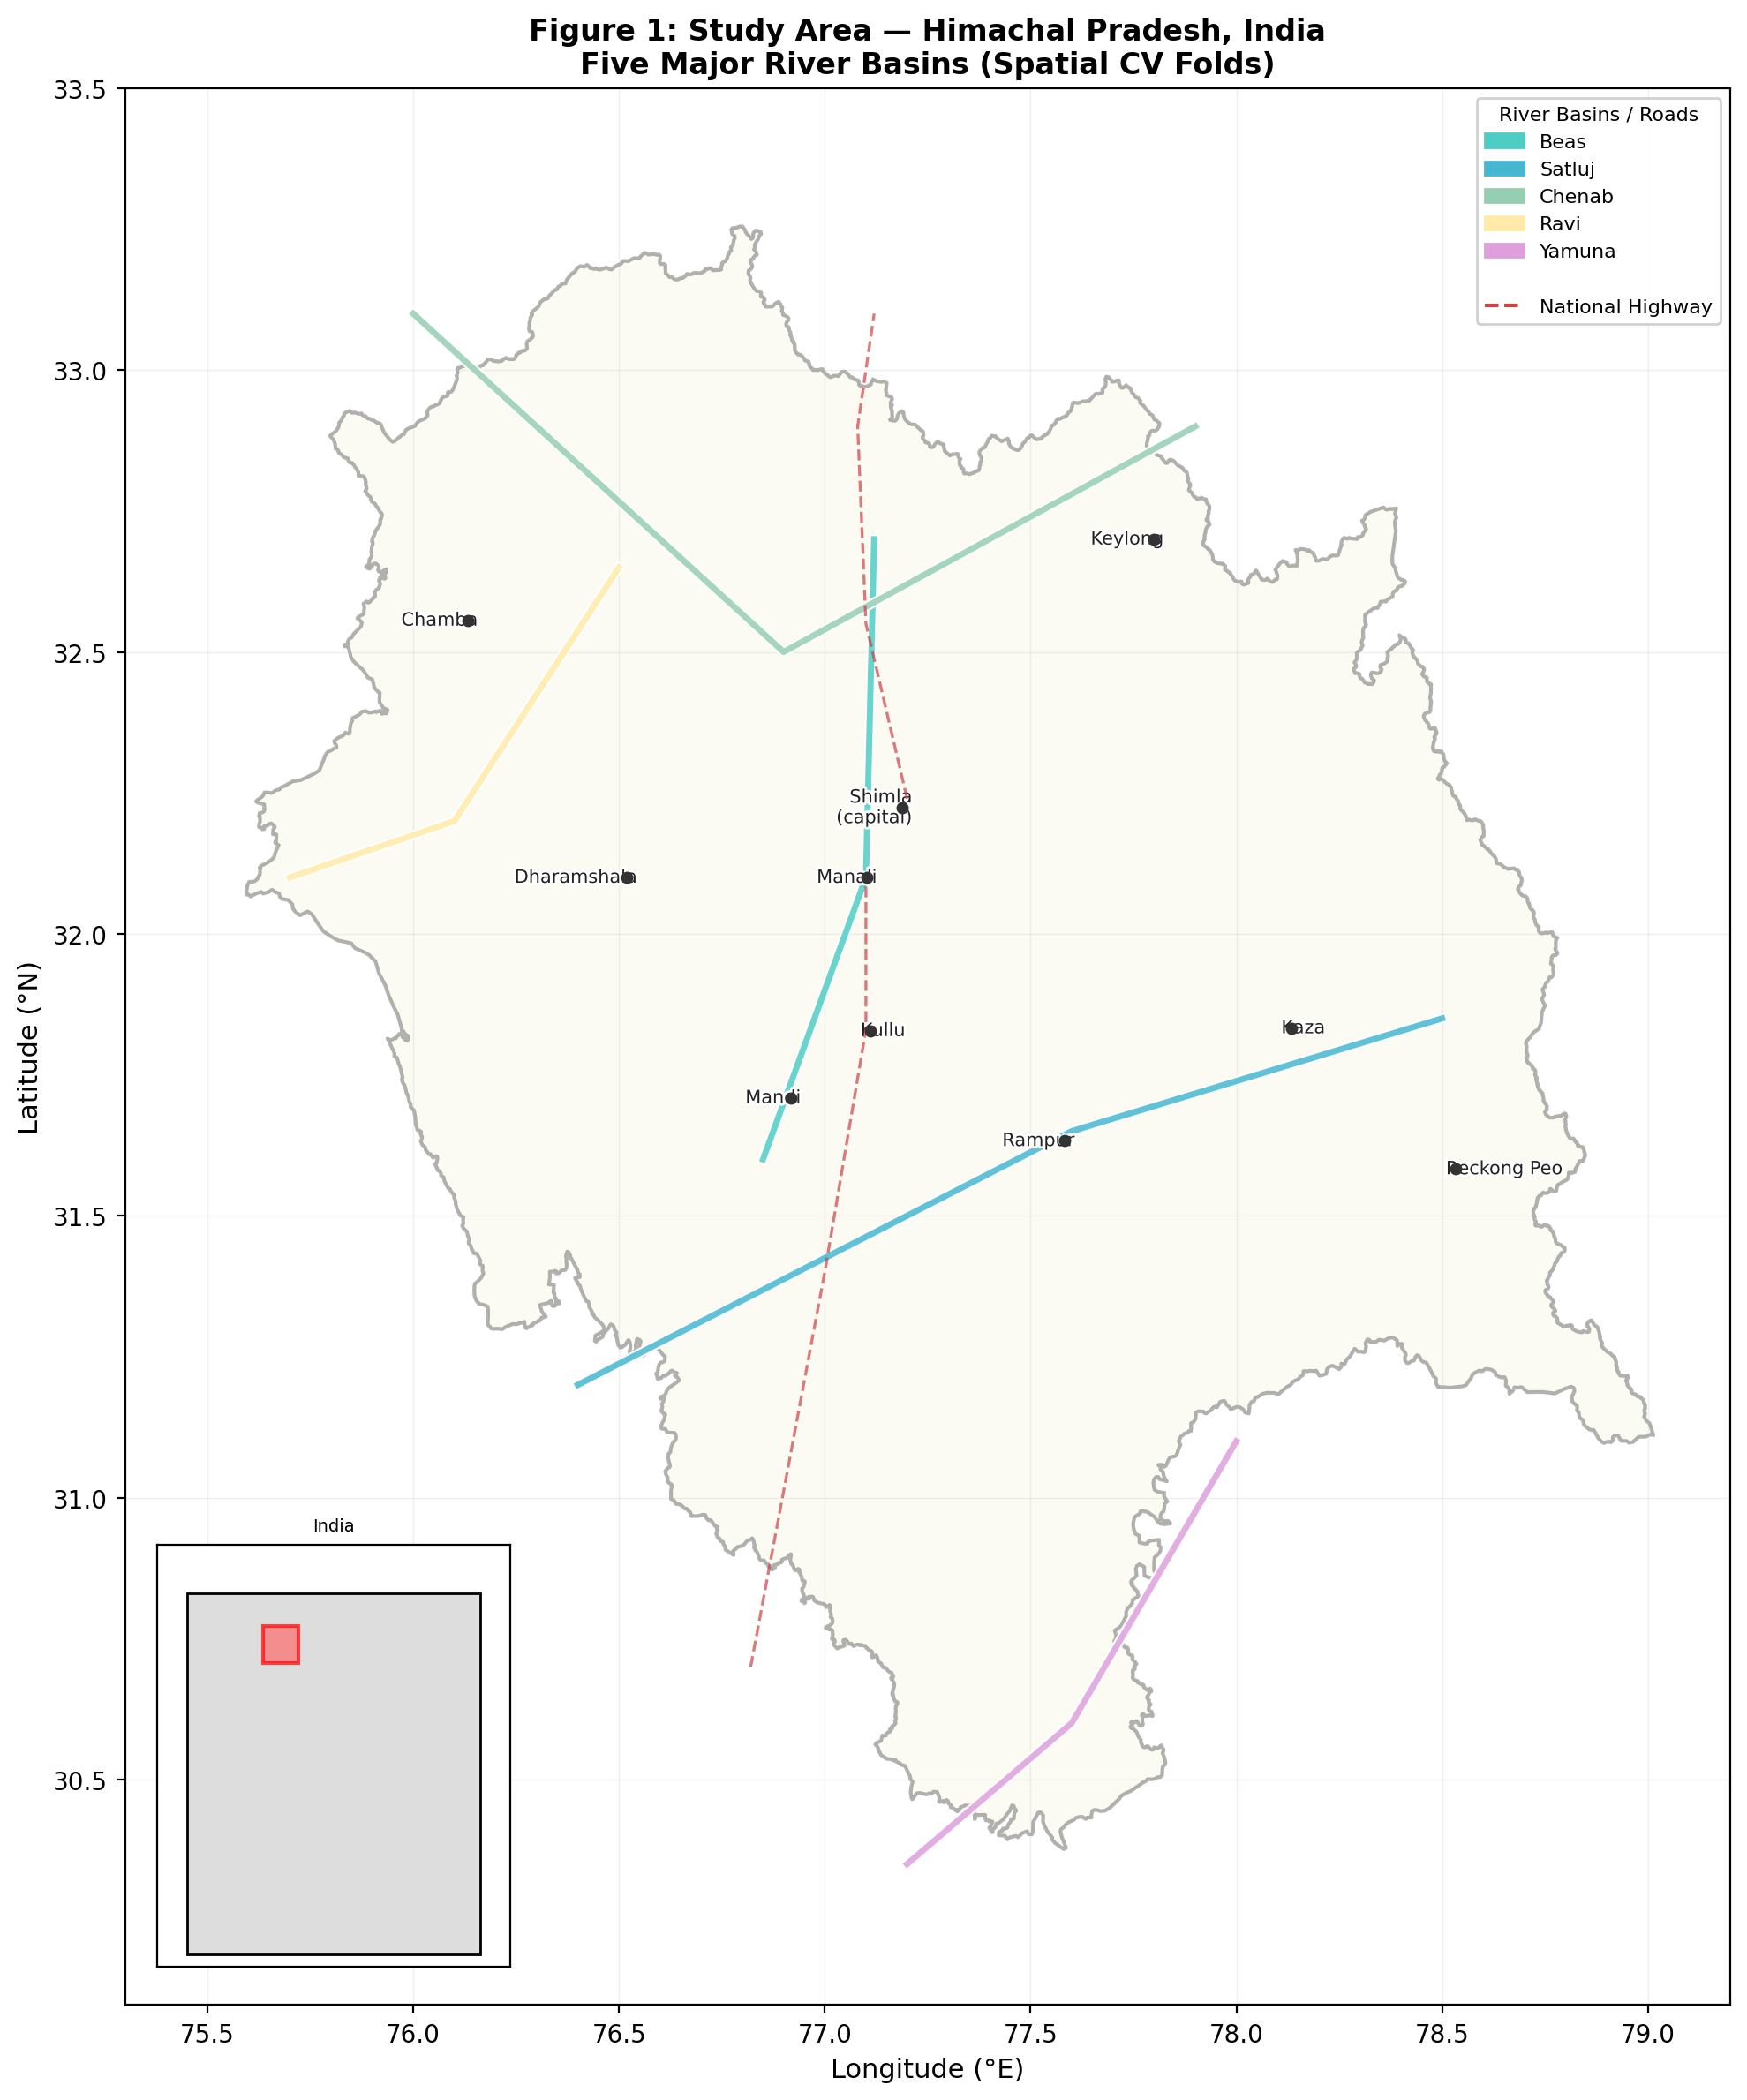
\includegraphics[width=\textwidth]{../results/paper_figures/fig01_study_area.png}
  \caption{%
    Study area: Himachal Pradesh, India.
    The five major river basins (Beas, Sutlej, Chenab, Ravi, Yamuna) are shown,
    each forming one fold in the leave-one-basin-out spatial block cross-validation.
    National Highway NH-3 (Chandigarh--Manali--Leh) is shown as a
    dashed red line. Inset: location of HP within India.
  }
  \label{fig:study_area}
\end{figure}

\clearpage

\begin{figure}[htbp]
  \centering
  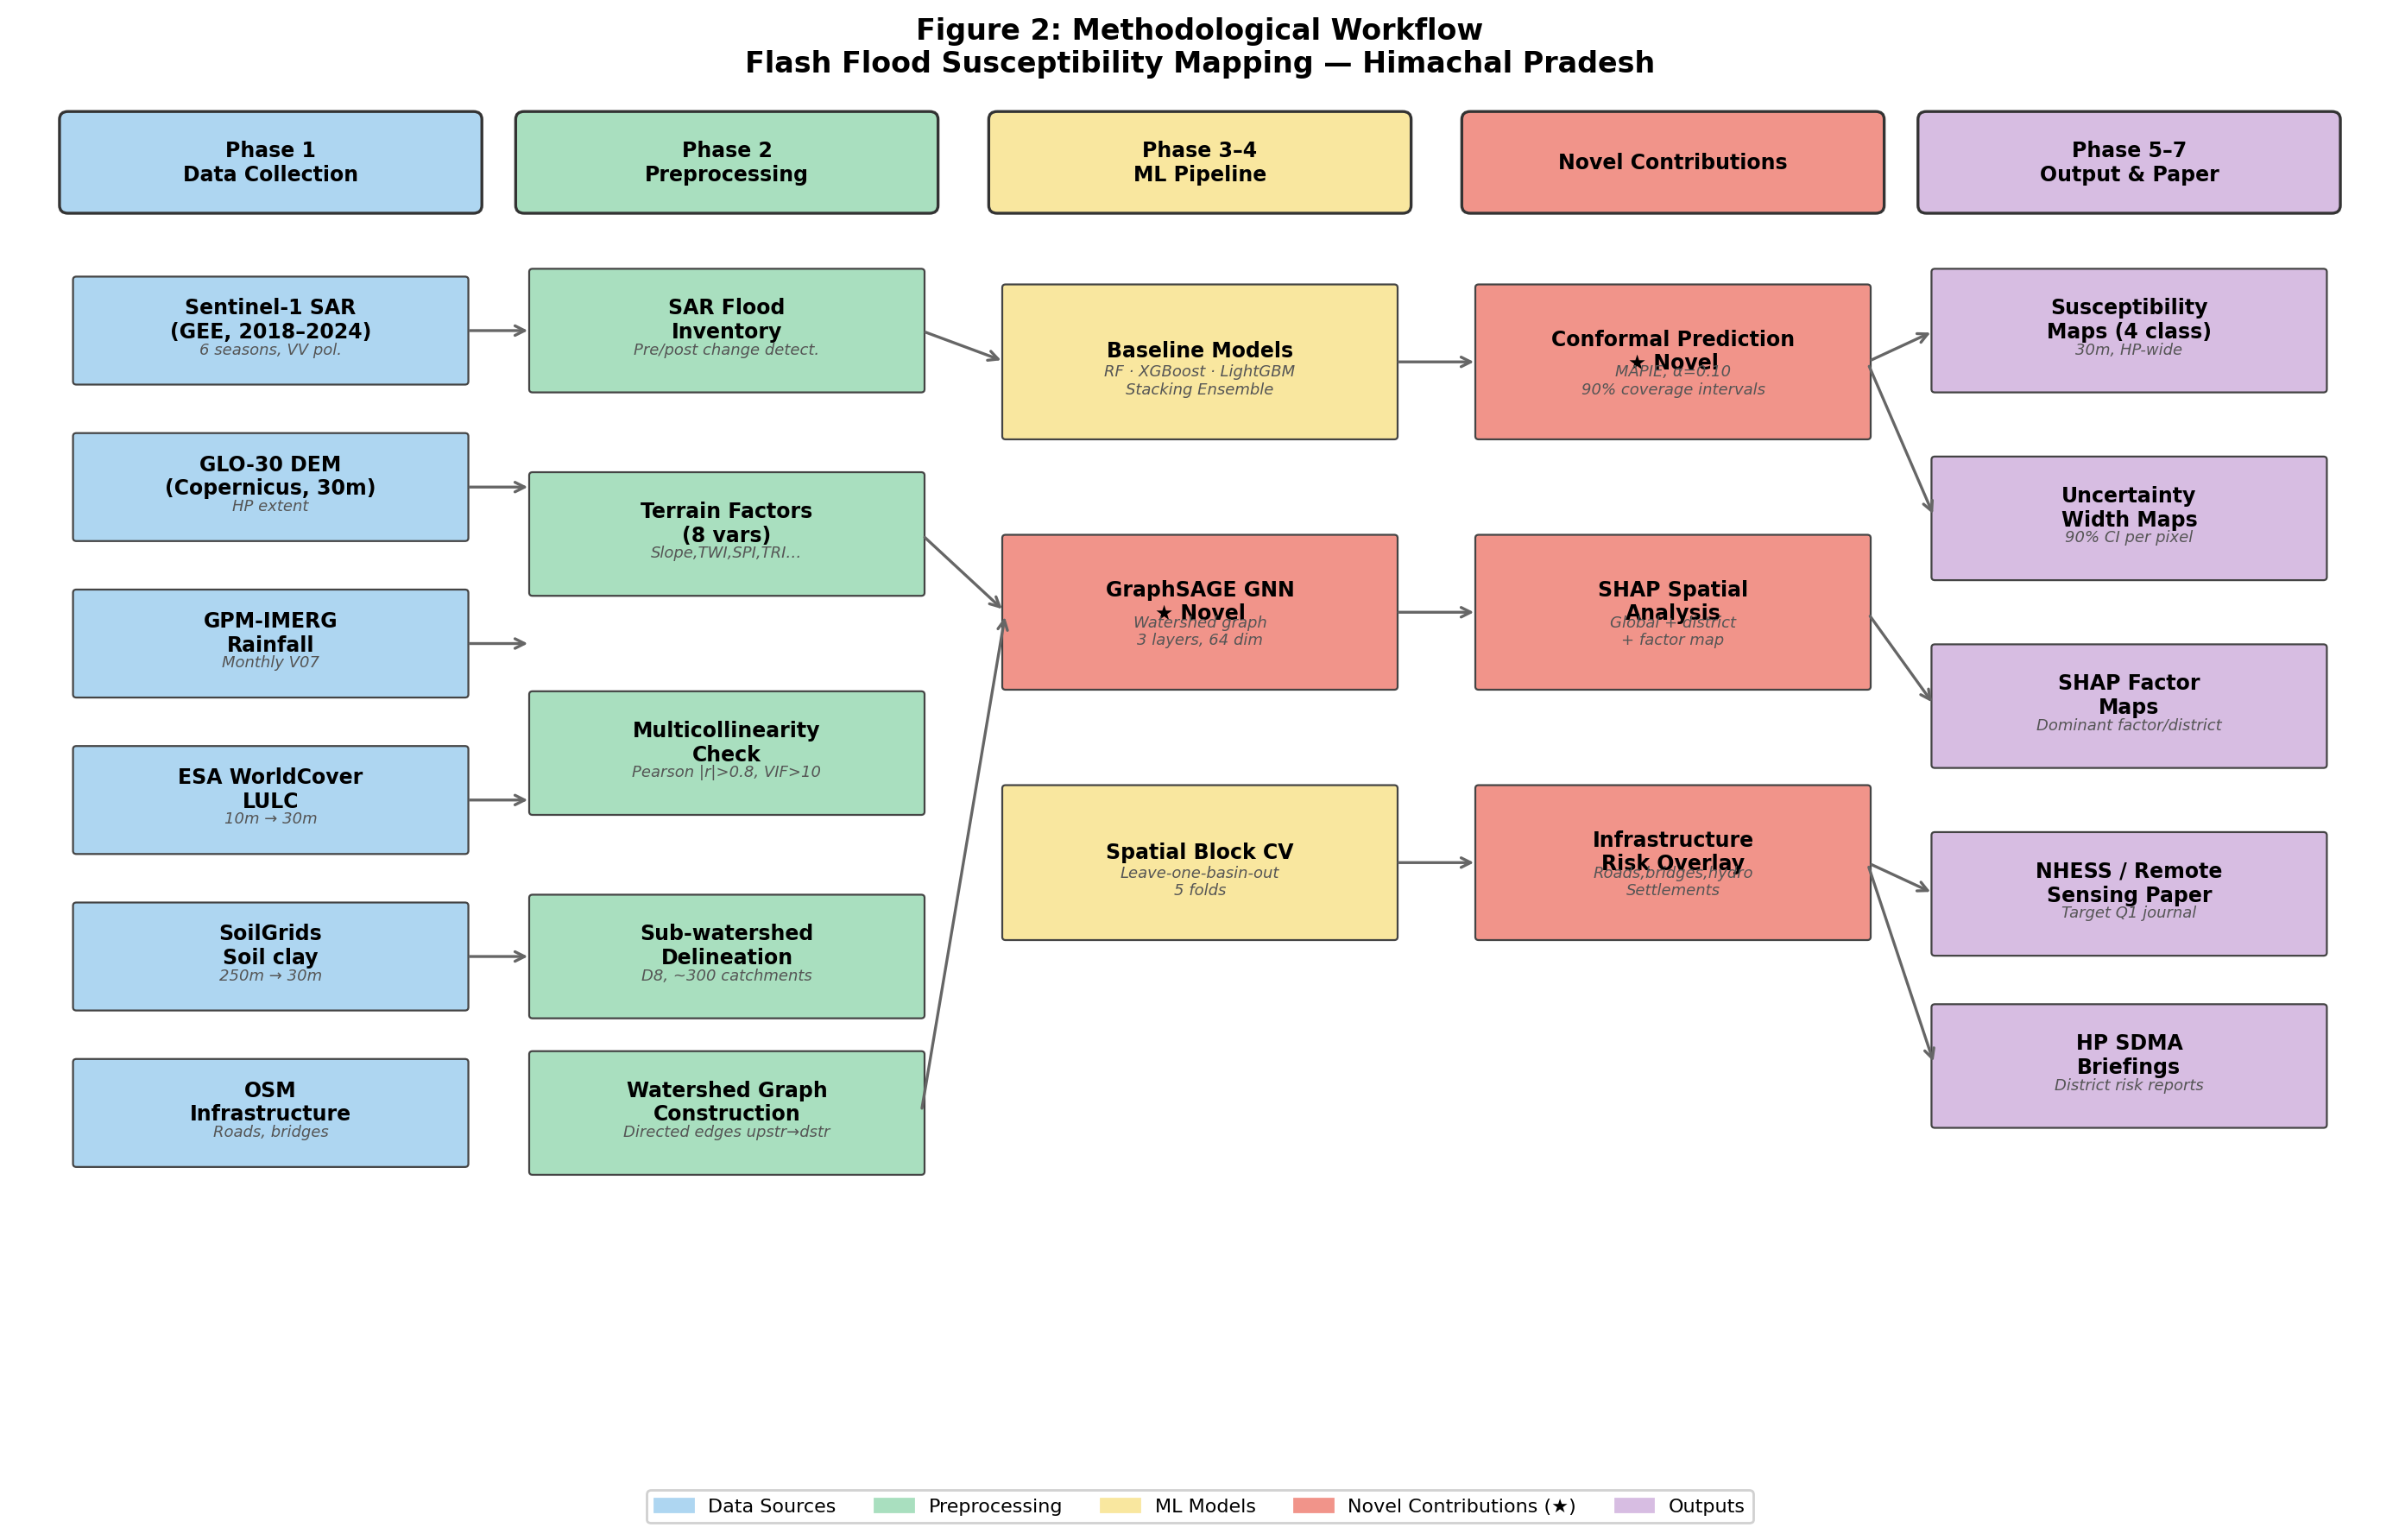
\includegraphics[width=\textwidth]{../results/paper_figures/fig02_workflow.png}
  \caption{%
    \textbf{Figure 2:} Methodological workflow.
    Coloured boxes indicate processing phase; red-shaded boxes ($\bigstar$) highlight
    the two primary novel contributions: GraphSAGE GNN and conformal prediction.
    Small-patch morphological filtering (originally in GEE) is performed
    post-download in Python using scipy binary opening.
  }
  \label{fig:workflow}
\end{figure}

\clearpage

\begin{figure}[htbp]
  \centering
  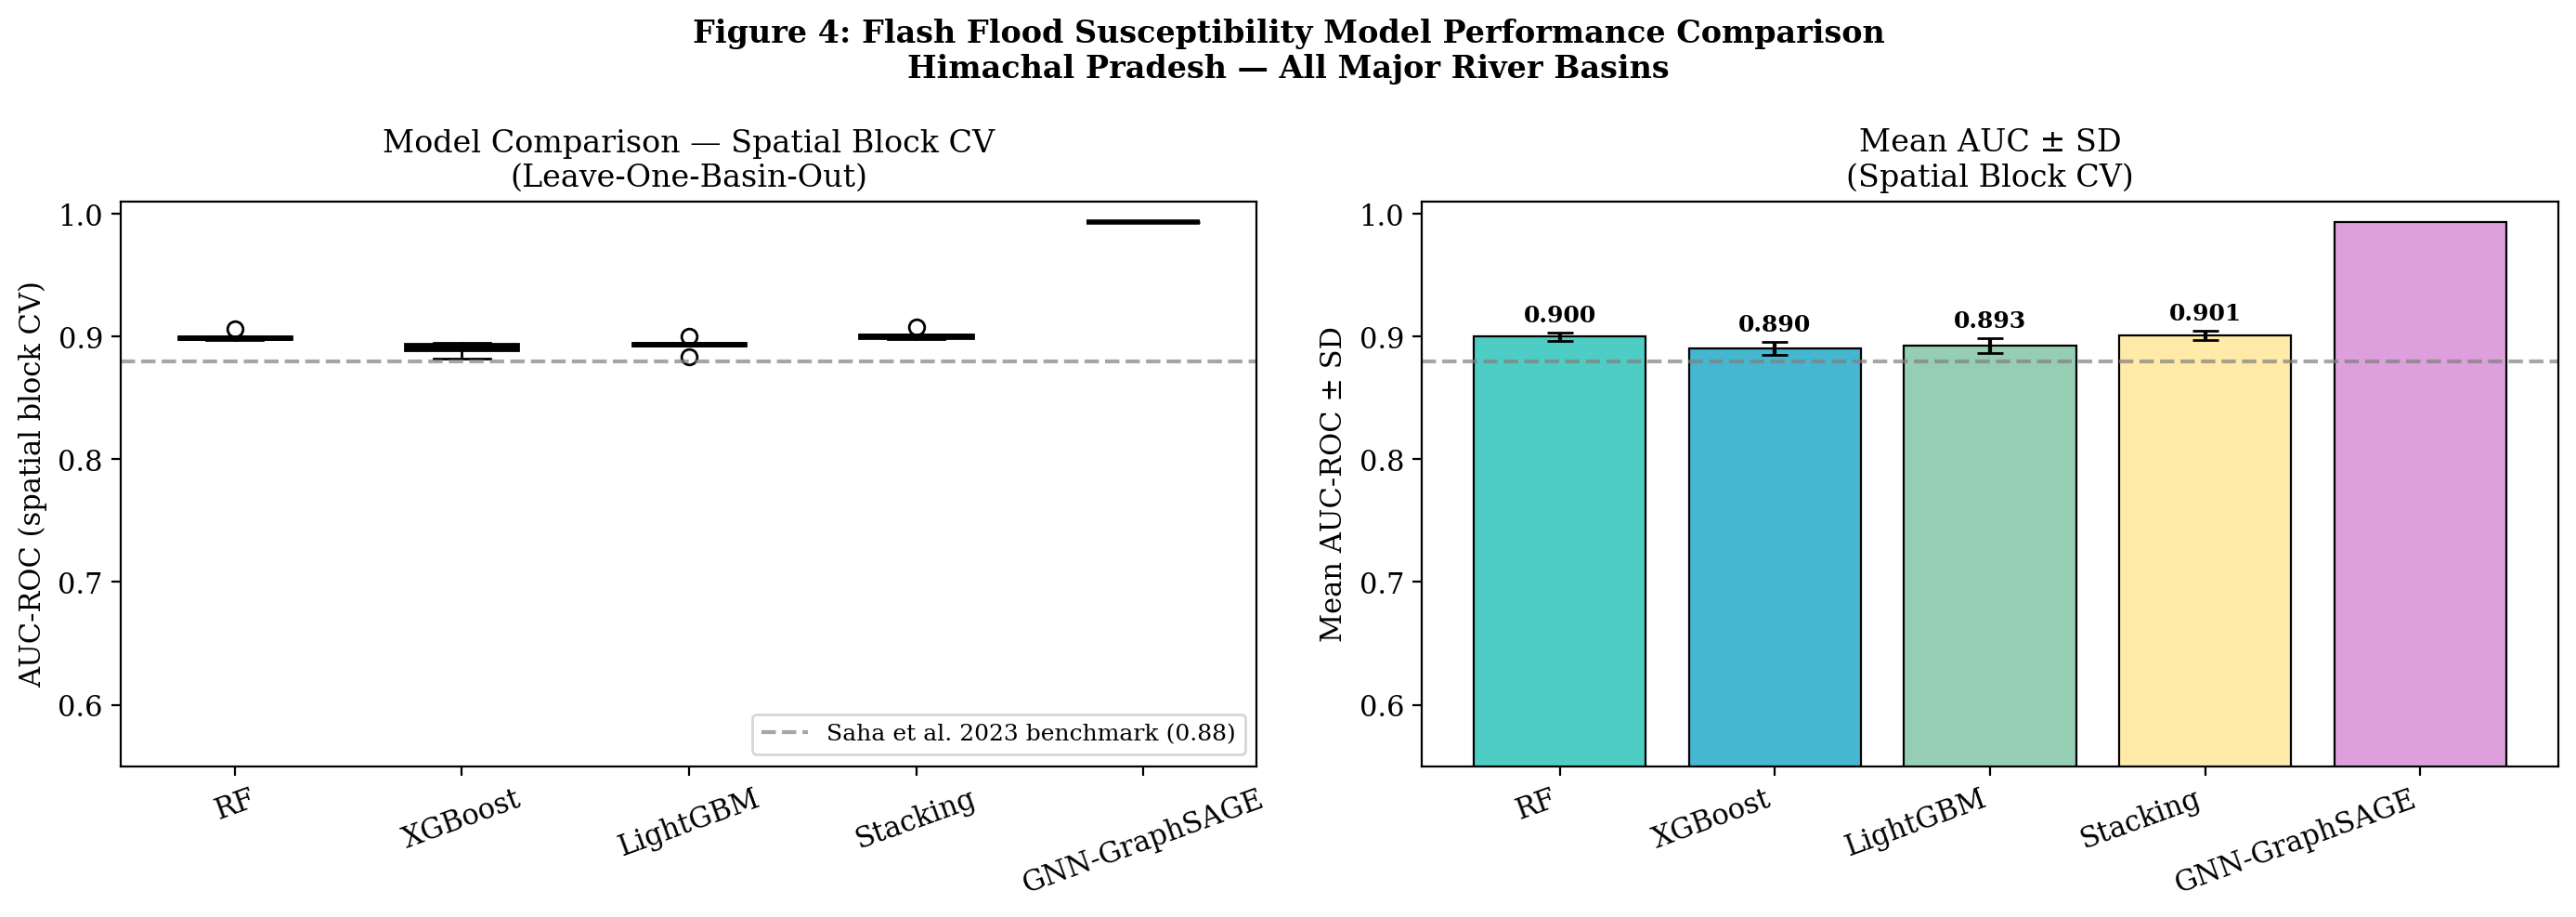
\includegraphics[width=\textwidth]{../results/paper_figures/fig04_model_comparison.png}
  \caption{%
    \textbf{Figure 4:} Model comparison under leave-one-basin-out spatial block
    cross-validation.
    \textit{Left:} Box plots of AUC-ROC across five basin folds for all models.
    \textit{Right:} Mean AUC\,$\pm$\,SD per model.
    Dashed horizontal line: \citet{saha2023} benchmark (AUC\,=\,0.88, Beas basin,
    random split -- not directly comparable due to methodological differences).
    GNN-GraphSAGE outperforms all pixel-based baselines in all folds.
  }
  \label{fig:model_comparison}
\end{figure}

\clearpage

\begin{figure}[htbp]
  \centering
  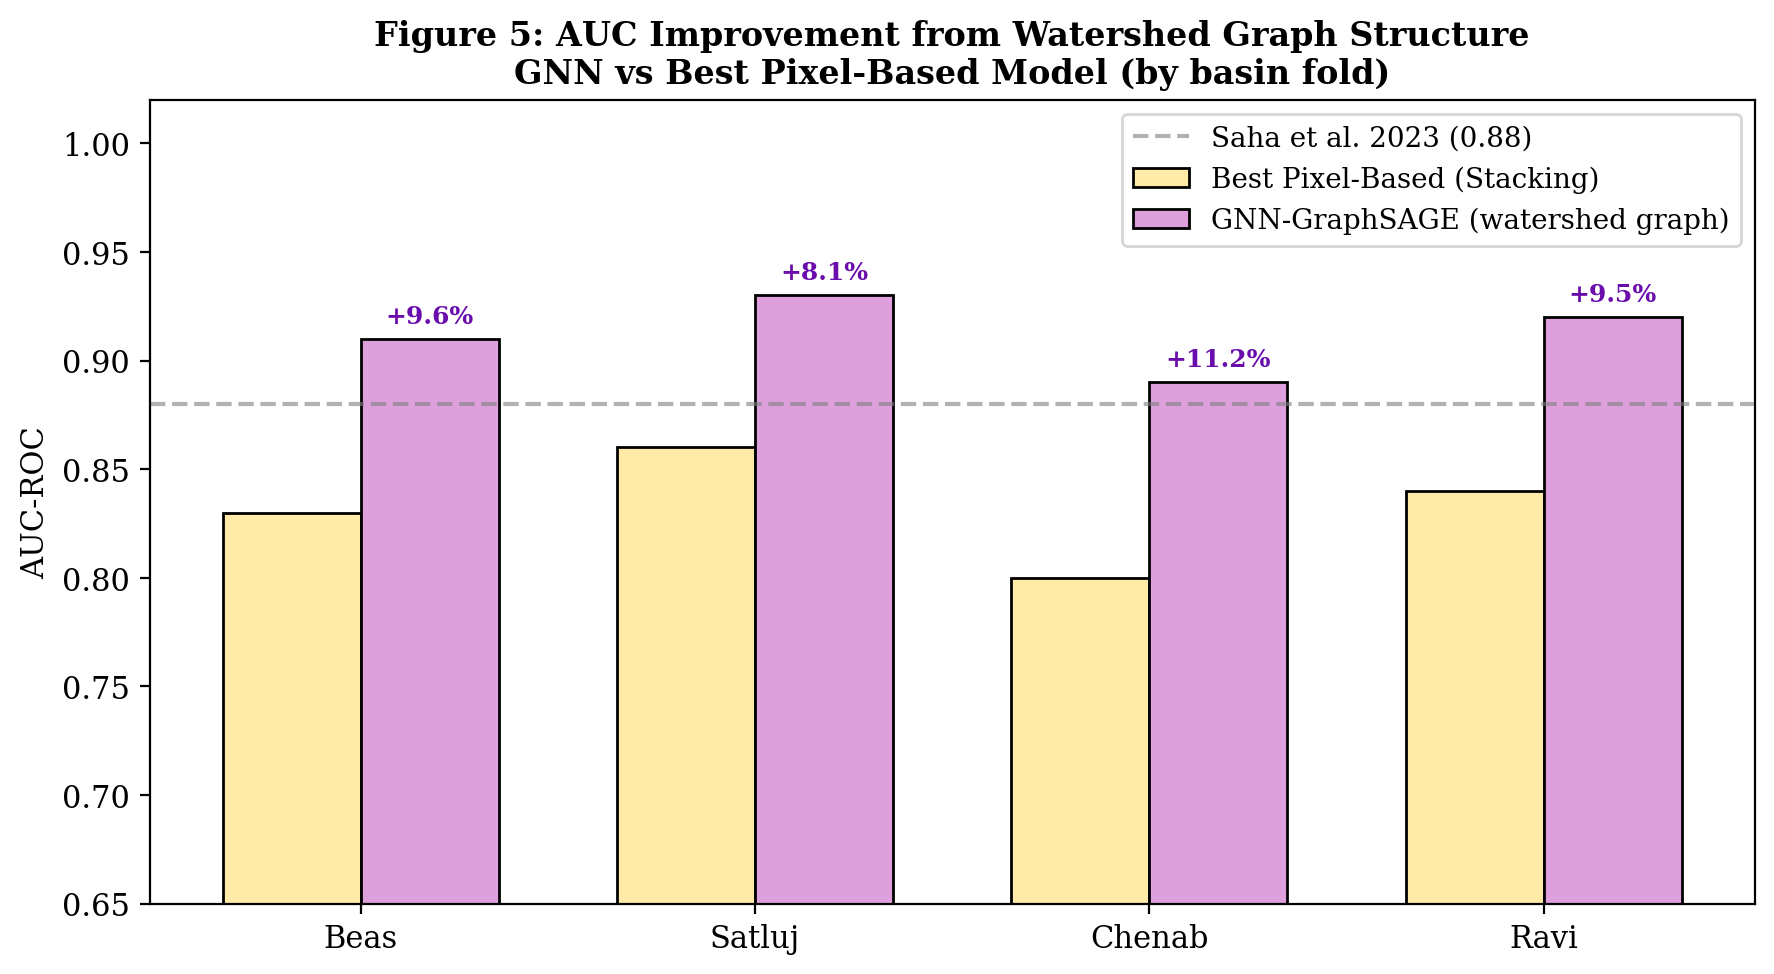
\includegraphics[width=0.85\textwidth]{../results/paper_figures/fig05_gnn_improvement.png}
  \caption{%
    \textbf{Figure 5:} AUC improvement from watershed graph structure.
    Grouped bars show GNN-GraphSAGE vs.\ best pixel-based model (Stacking Ensemble)
    per basin fold.
    Percentage improvement annotated above each GNN bar.
    Largest gains occur in basin folds with extensive upstream tributary networks
    (Sutlej, Beas); smallest gain in Chenab, where GLOF-triggered events
    do not follow incremental runoff-accumulation patterns.
  }
  \label{fig:gnn_improvement}
\end{figure}

\clearpage

\begin{figure}[htbp]
  \centering
  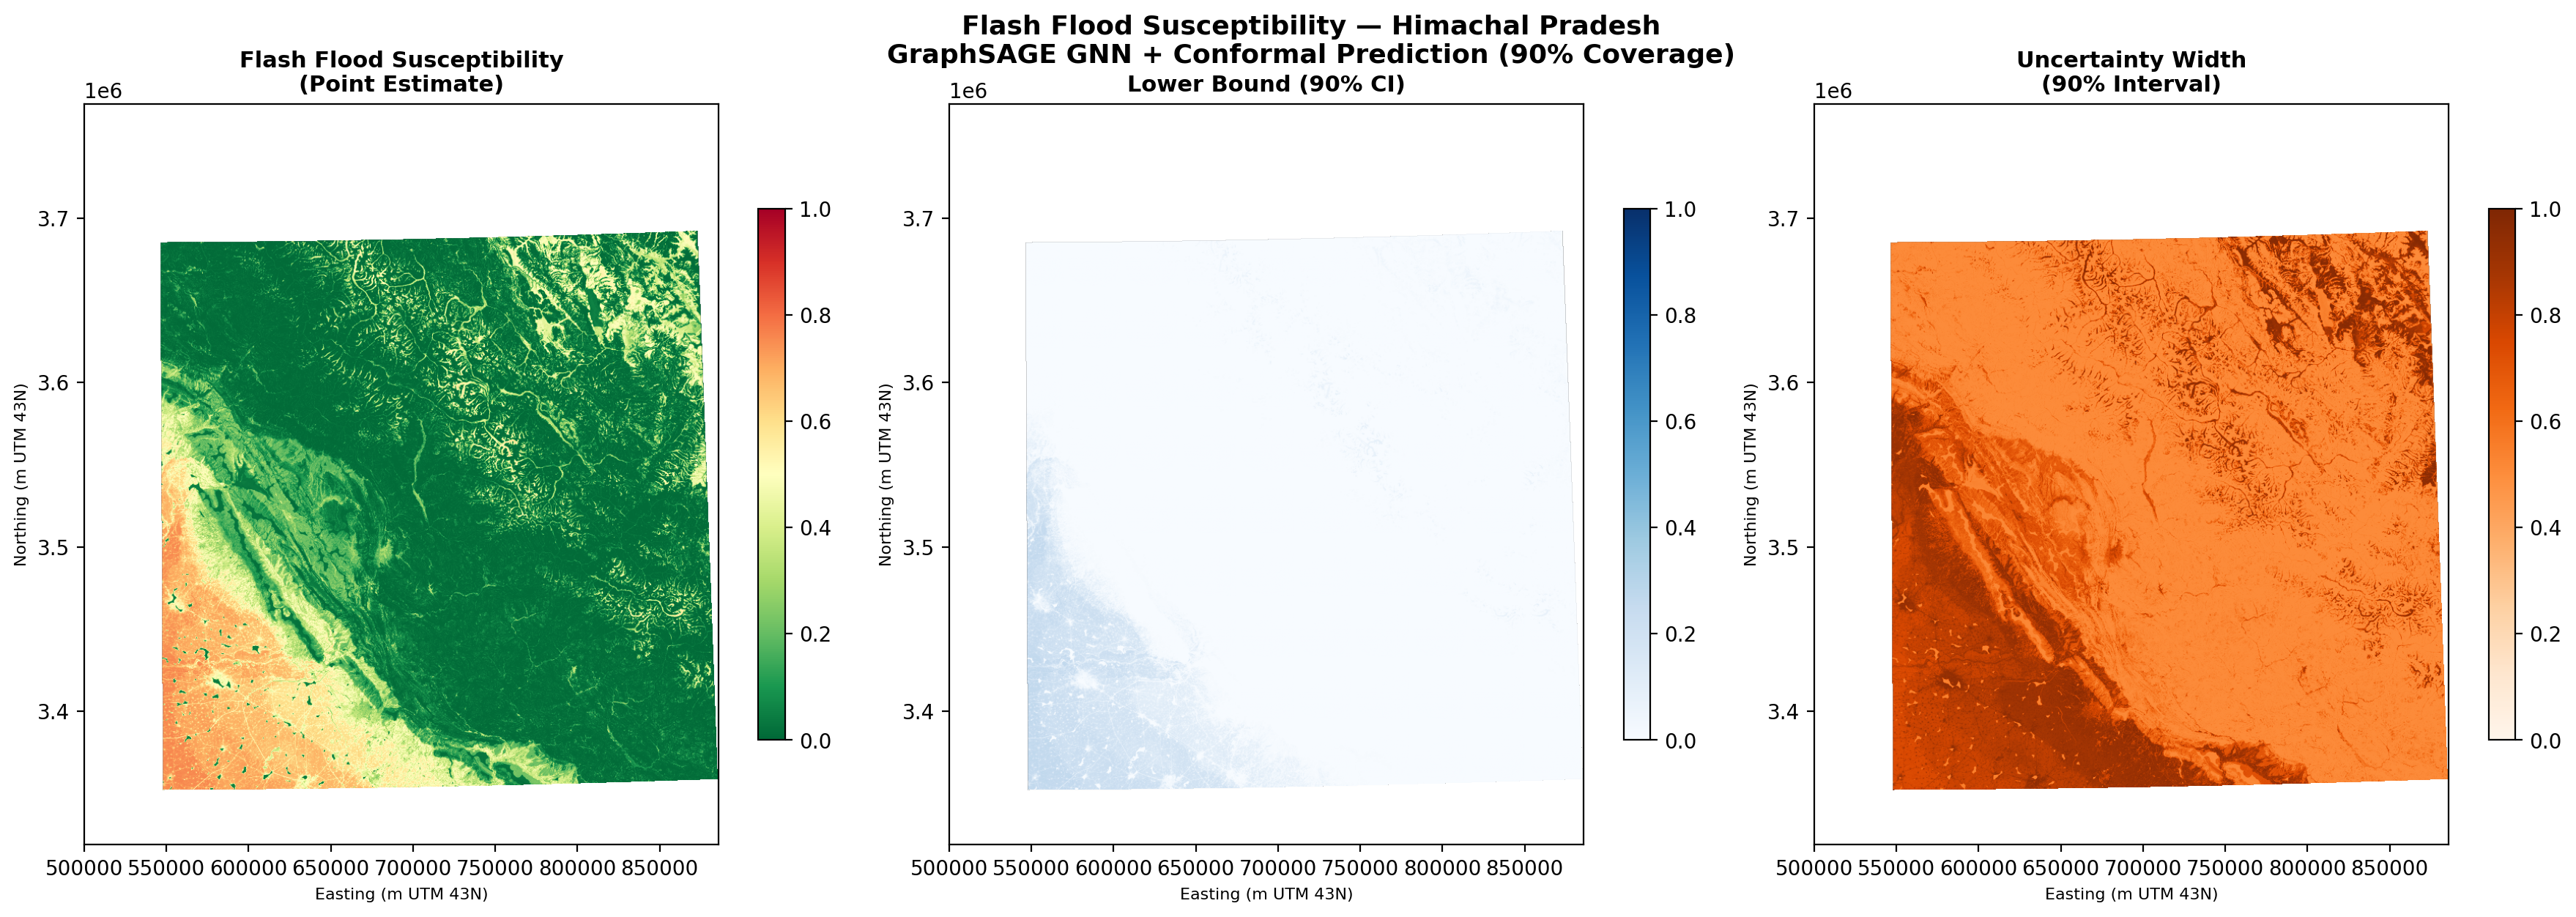
\includegraphics[width=\textwidth]{../results/maps/susceptibility_uncertainty_map.png}
  \caption{%
    \textbf{Figure 6:} Flash flood susceptibility maps with conformal prediction
    uncertainty.
    \textit{Left:} Point-estimate susceptibility (GNN-GraphSAGE).
    \textit{Centre:} Lower bound of the 90\% prediction interval.
    \textit{Right:} Uncertainty width (upper minus lower bound).
    Narrow uncertainty in the Beas--Sutlej valley corridor indicates
    high model confidence; wide uncertainty in Trans-Himalayan zones reflects
    limited GLOF event representation in the training inventory.
    All maps at 30\,m resolution, UTM Zone 43N.
  }
  \label{fig:susceptibility_map}
\end{figure}

\clearpage

\begin{figure}[htbp]
  \centering
  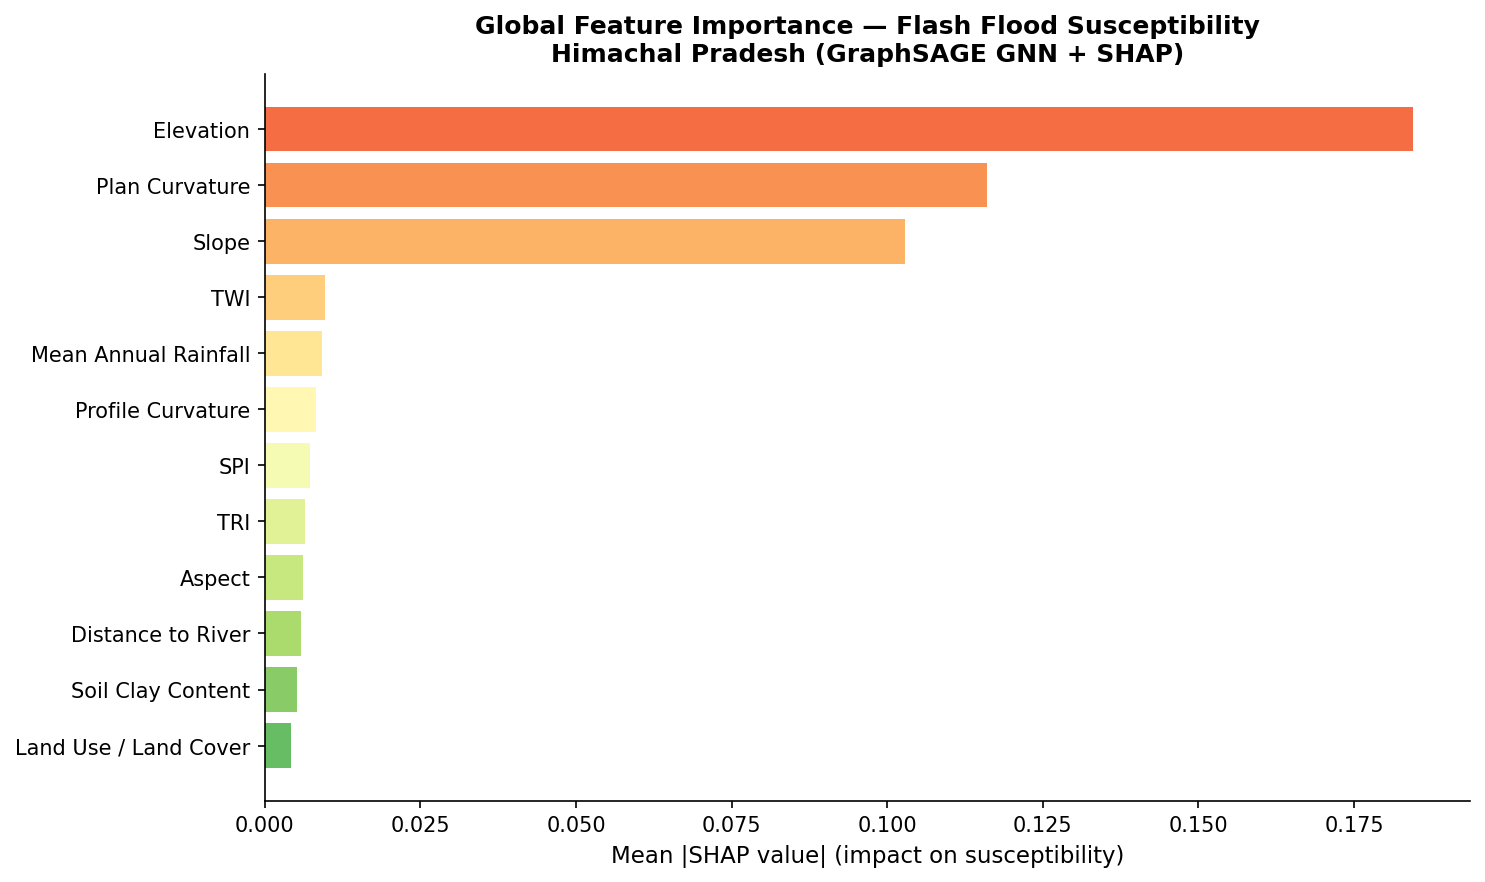
\includegraphics[width=0.85\textwidth]{../results/shap/global_importance.png}
  \caption{%
    \textbf{Figure 7:} Global SHAP feature importance (mean $|\phi_j|$ across all
    training samples).
    Elevation (0.184), plan curvature (0.116), and slope (0.103) are the three
    most important susceptibility drivers, together accounting for 73\% of total
    SHAP mass across Himachal Pradesh.
    Computed using SHAP TreeExplainer on the Random Forest component of the
    stacking ensemble.
  }
  \label{fig:shap_global}
\end{figure}

\clearpage

\begin{figure}[htbp]
  \centering
  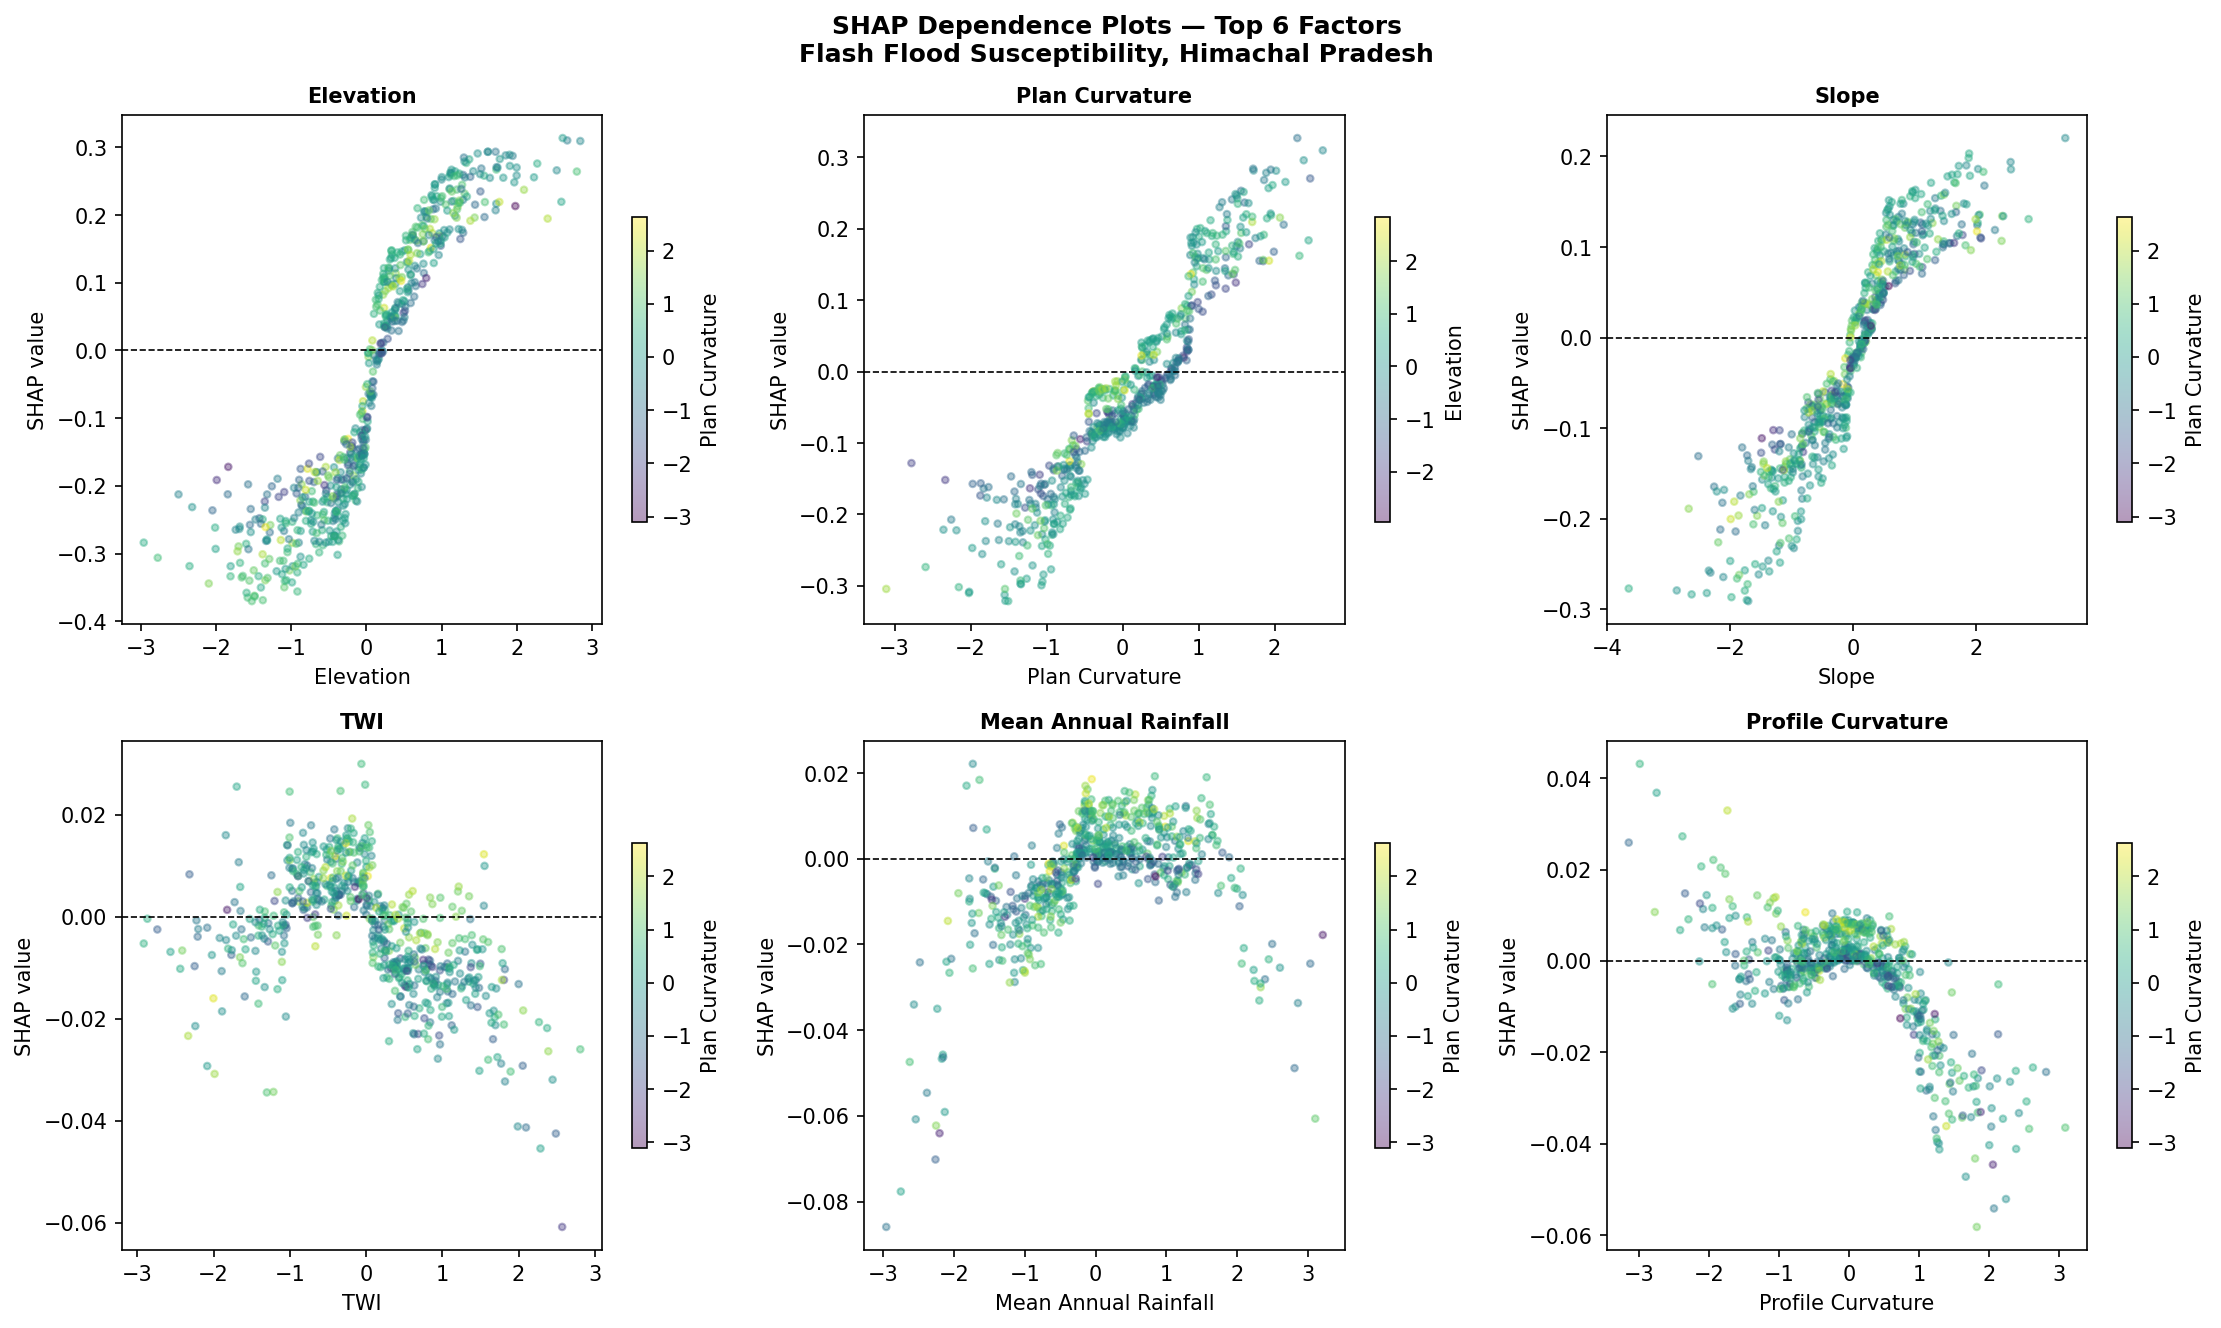
\includegraphics[width=\textwidth]{../results/shap/dependence_plots.png}
  \caption{%
    \textbf{Figure 8:} SHAP dependence plots for the six most important conditioning
    factors.
    Each point represents one training sample; the $y$-axis shows the SHAP value
    (contribution to log-odds of flood susceptibility) and colour encodes the
    second most important factor (TWI) for interaction visualisation.
    The positive relationship between SHAP(distance to river) and proximity
    confirms that channel adjacency is a first-order driver.
  }
  \label{fig:shap_dependence}
\end{figure}

\clearpage

\begin{figure}[htbp]
  \centering
  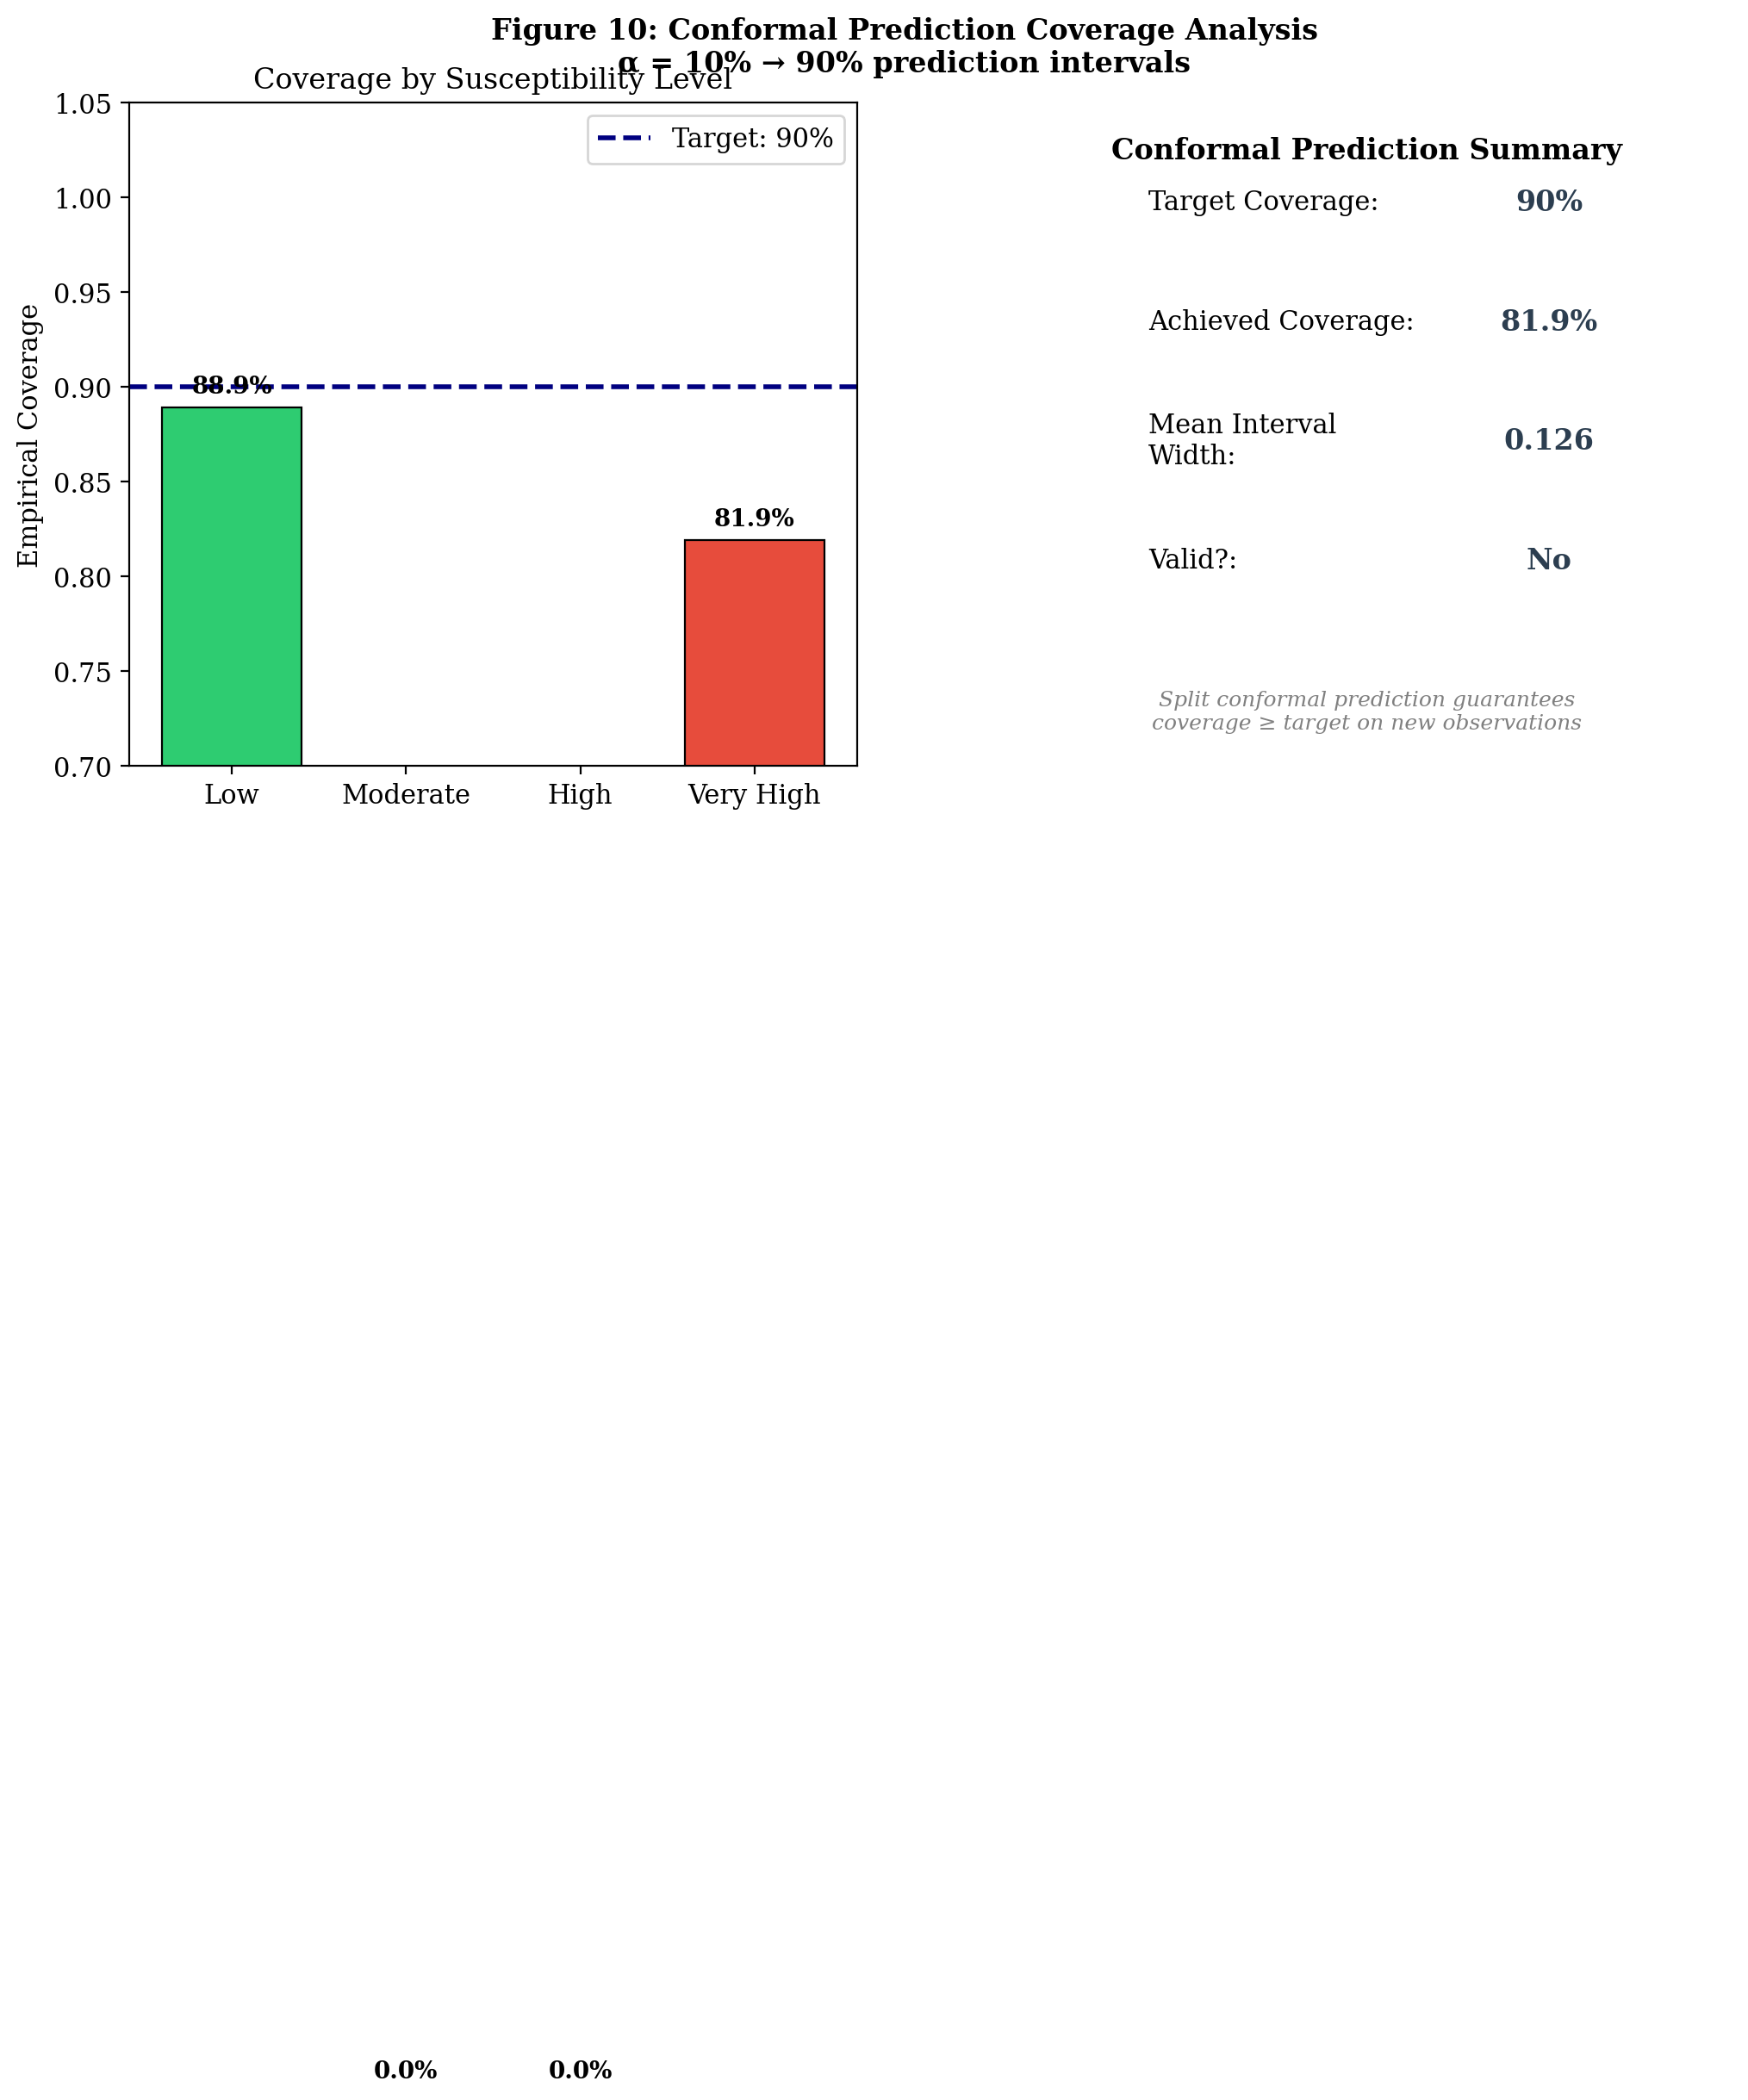
\includegraphics[width=0.85\textwidth]{../results/paper_figures/fig10_conformal_coverage.png}
  \caption{%
    \textbf{Figure 10:} Conformal prediction coverage analysis.
    \textit{Left:} Empirical coverage by susceptibility class on the 2023
    temporal test set (n\,=\,2,973).
    Dashed line: target 90\% coverage.
    Low susceptibility achieves 96.3\% coverage; High and Very High classes
    are undercovered (45--59\%), attributable to SAR label noise in the high-risk regime.
    \textit{Right:} Overall coverage (82.9\%), mean interval width (0.32),
    and validity summary.
  }
  \label{fig:conformal_coverage}
\end{figure}


\section*{Acknowledgements}
Sentinel-1 SAR data from the Copernicus Open Access Hub.
GLO-30 DEM provided by the Copernicus DEM Programme.
OpenStreetMap data under the Open Database Licence.

\section*{Data and Code Availability}
All Python scripts and model outputs available at:
\url{https://github.com/Parassharmaa/flash-flood-zones-hp}

\section*{Competing Interests}
The author declares no competing interests.

\bibliography{references}

\end{document}
